\documentclass[12pt,a4paper]{report}

\usepackage{subfigure,epsfig,amstext,floatfig,alltt,fancyhdr,setspace,amsmath}
\usepackage{epstopdf}
\usepackage{float}
\usepackage{graphicx}
\include{macros}
\initfloatingfigs

%%% helps to discourage hyphenation 10000 for no hyphens but dodgy line lengths%%%
\hyphenpenalty=5000
\tolerance=1000

% sets all the margins to be the correct size for thesis

%%%%%%% FINAL THESIS MARGINS  %%%%%%%%%
\setlength{\oddsidemargin}{1.46cm}
\setlength{\evensidemargin}{-0.04cm}
\setlength{\textwidth}{14.5cm}
\setlength{\topmargin}{-0.54cm}
\setlength{\textheight}{21.9cm} 
\renewcommand{\hoffset}{0cm}
\renewcommand{\voffset}{0cm}
%%%%%%%%%%%%%%%%%%%%%%%%%%%%%%%%%%%%%%%
\setcounter{secnumdepth}{3}
\setcounter{tocdepth}{3}
\DeclareMathAlphabet{\mathpzc}{OT1}{pzc}{m}{it}

%% In the beginning ....
\begin{document}
%% First do introductory stuff - leave this as pagestyle empty until after
%% the table of contents

%\title{
\pagestyle{empty}

\begin{center}
\LARGE
%\vspace*{2cm}
{\bf Neutron Skin Measurement of Tin Isotopes}

\vspace{1cm}
%\begin{figure}[!ht]

\begin{figure}[ht]
\begin{center}
%
\epsfig{file=crest.png,width=0.3\linewidth}

\includegraphics[scale=0.4]{pictures/eps/crest.eps}
\end{center}
\end{figure}

\large
{\it Dominika Glowa}

\vspace{9cm}
\normalsize
%\begin{center}        
Doctor of Philosophy\\
The University of Edinburgh\\
August 2015\
%for the degree of Doctor of Philosophy\\
%to the\\ 
%University of Edinburgh

June 2014
\end{center}
%\maketitle     


%\ \newpage		% Newpage needed if doing double sided.

%% Include abstract - use separate parskip for this and then set parskip for
%% rest of thesis.
%\pagestyle{plain}

%-----------------------------------------------------------------------------

\pagestyle{fancy}
\fancyhead{} %clear all fields
\renewcommand{\headheight}{28pt}
\cfoot{}
\fancyfoot[LE,RO]{\thepage}

\renewcommand{\chaptermark}[1]{\markboth{\chaptername \ \thechapter.\ #1}{}} 
\renewcommand{\sectionmark}[1]{\markright{\thesection.\ #1} {}}

\fancyhead[LE]{\small \slshape \leftmark}      % Chapter in the right on even pages
\fancyhead[RO]{\small \slshape \rightmark}     % Section in the left on odd pages
\renewcommand{\headrulewidth}{0.3pt}    % Width of head rule

%-----------------------------------------------------------------------------


\pagenumbering{roman}
\setcounter{page}{1}

\onehalfspacing

\addcontentsline{toc}{chapter}{Abstract}
\chapter*{Abstract}
\noindent

\indent Heavy atomic nuclei are thought to have proton and neutron radial distributions which have different sizes. This difference is usually quantified in terms of a neutron skin (r$_{np}$), defined as the difference between the root mean square radii of the neutrons and proton radial distributions ($r_{np} = r_{n}^{2} - r_{p}^{2}$). The nature or even existence of the neutron skin is currently not well established. Different nuclear theories give different predictions for the neutron skin thickness of a typical heavy nucleus ranging from 0.05 to 0.35 fm. Accurate measurement of the properties of the neutron skin would be a powerful constraint to differentiate between models of nuclear structure and improve our knowledge of the basic Equation Of State (EOS) for neutron rich matter. Particularly, the rate at which the neutron skin thickness changes across an isotopic chain of nuclei gives a tight constraint on the EOS and is also amenable to experimental determination with small systematic error. Improving our knowledge of the EOS for neutron rich matter is a crucial step to a deeper understanding of nuclear structure and of compact astrophysical objects such as neutron stars. This thesis describes the first measurement of neutron skin  along an isotopic chain. The neutron skin is measured through the study of pions coherent photoproduction from nuclei. 

\indent This experiment was carried out in the A2 hall of the MAMI facility in Mainz, Germany in October 2012.  The incident photon beam comprised energy tagged photons in the range of $E_{\gamma}$=150-800 MeV with an intensity of ~10$^{8}$ sec$^{-1}$. Experimental data was obtained for three different tin targets, $^{116}Sn$, $^{120}Sn$ and $^{124}Sn$. The products from the resulting photoreactions were measured in the Crystal Ball detector and in the TAPS calorimeter systems, with track and particle identification information for charged particles provided by a multi wire proportional chamber (MWPC) and a particle identification detector (PID).

\indent The experiment provides the first information on the evolution of the neutron skin thickness along an isotopic chain using an electromagnetic probe. The results are compared with a range of theoretical models and previous data from strongly interacting probes. The new data provides an important experimental constraint on the basic properties of the EOS in atomic nuclei.

\indent

\vspace{10mm}
\normalsize


%\ \newpage		% Newpage needed if printing double sided.

%\addcontentsline{toc}{chapter}{Declaration}
%\chapter*{Declaration}

\normalsize
Except where otherwise stated, the research undertaken in this thesis
was the unaided work of the author. Where the work was done in collaboration
with others, a significant contribution was made by the author.


\vspace{20mm}
\hfill {\it A. Hollingsworth}

\hfill May 2011




%\ \newpage		% Newpage needed if printing double sided.

\singlespacing

%\ \newpage		% Newpage needed if printing double sided.

%\addcontentsline{toc}{chapter}{Contents}
%\tableofcontents

%\ \newpage		% Newpage needed if printing double sided.
%\ \newpage		% Newpage needed if printing double sided.

%\addcontentsline{toc}{chapter}{List of figures}
%\listoffigures

%\ \newpage		% Newpage needed if printing double sided.

%\addcontentsline{toc}{chapter}{List of tables}
%\listoftables
  
%\ \newpage		% Newpage needed if printing double sided.
%\ \newpage		% Newpage needed if printing double sided.

\clearpage % this command stops table page becoming page 1


%% Now the body of the text - note that parskip has to be reset after the TOC

\onehalfspacing
\pagenumbering{arabic}

\setcounter{page}{1}
%% Add chapters here %%
%\chapter{Prologue}

\indent The composition of the world around us has been of unflagging interest to men throughout history; the earliest known records attempting to explain the composition of matter date back to antiquity. However it was only in 1911 when Rutherford formulated the theory of atomic nucleus. Ever since this discovery the research into internal structure of a nucleus accelerated. Various experimental techniques have been developed to determine the size and shape of nuclei of different elements. As a result of numerous test employing methods such as electron scattering and x-ray spectroscopy the charge distribution in a nuclei has been estimated to $\sim0.01\%$ accuracies \cite{devires}. Despite a huge success of those experimental methods in determining the proton's arrangement within a nucleus they proved to be ineffective to test the neutron distributions, as the electrons only interact with the charge in the nucleus. Strongly interacting probes such as protons, antiprotons and alpha particles have given inconsistent determinations of the nature of the neutron distributions in nuclei. The theoretical models describing these processes are still heavily subjected to large uncertainties in the description of strong interactions \cite{claire}. Currently it is not well established how the distributions of neutrons differ from protons in the nucleus.

\indent According to theoretical predictions of nuclear structure, nuclei with similar numbers of protons and neutrons have almost no difference between r.m.s. radii of charge and matter distributions. However, this situation is predicted to change with increasing mass number. It is predicted that for nuclei with the number of neutrons being much greater than the number of protons, excess neutrons form a skin around the nucleus. This neutron skin is defined as:

\begin{equation}
\Delta R = r_{n} - r_{p}
\end{equation}
where $r_{n}$ and $r_{p}$ are the r.m.s. radii of neutron and proton respectively \cite{roca}. Having $\Delta$R determined accurately from experiment for a range of nuclei will provide a stringent constraint on current nuclear structure theories. There are many different theoretical models in common use, which predict very different values for the neutron skin; and experimental measurements could provide a mean of verification of the validity of those models. Furthermore, an accurate measurement of the neutron skin will have far reaching implications in the field of nuclear physics. Currently, poorly established parameters in the equation of state for the neutron rich matter show a largely model independent linear dependence on the size of the neutron skin. Precise measurement of the neutron skin will put constraints on these parameters, which in turn will provide basis for understanding physics of neutron stars, such as the mass-radius relationship of low mass neutron stars and modified URCA cooling.

\indent Neutron skin measurements have been performed with strongly interacting probes before. The obtained data were strongly affected by many-body strong interaction effects that made the analysis and interpretation of the results ambiguous and difficult to draw binding conclusions from. The experiment involving proton scattering data fitted with different neutron skin thicknesses concluded with data being unable to determine the size or even the existence of the neutron skin \cite{pike}.

\indent The use of photons to study neutron skin potentially allows for much more accurate measurements than strongly interacting probes. The strength of photon's electromagnetic interactions is very weak and as such they are not affected by the initial state interactions (ISI) and many-body interaction effects do not complicate the interpretation of the obtained data. Furthermore, the electromagnetic interactions are far better understood than strong interactions, and therefore, the results obtained with the use of electromagnetic probes are less susceptible to systematic effects in their theoretical interpretation \cite{claire}.

\indent Coherent $\pi^{0}$ photoproduction takes place when a photon interacts with a target nucleon and as a result a $\pi^{0}$ meson is emitted, A($\gamma,\pi^{0}$)A. Even though the photons, being weakly interacting and unaffected with ISI, the produced pions are strongly interacting particles and therefore the effect of final state interactions (FSI) with the nucleus has to be accounted for. It has been shown previously that the strength of the FSI scales with pion energy and that the pion-nucleus scattering cross section is dominated by the $\Delta$(1232) resonance corresponding to the pion energy of $\sim165MeV$ . Pions with energies well away from the peak of the resonance have smaller probability of interaction with the nucleus. The study of coherent $\pi^{0}$ photoproduction provides therefore a unique way to test not only nuclear matter distribution but pion-nucleus interactions as well.

\indent The main objective of the experiment presented in this thesis is however, to use the coherent $\pi^{0}$ photoproduction as a means to study the nuclear matter distribution of three stable tin isotopes in order to determine how the neutron skin thickness evolves with the mass number. The theoretical background to the experiment and methodology are presented in the next chapter. The experimental details are presented in the subsequent chapter. Then follows the summary of the current state of knowledge and a short description of possible implications of the results presented in this thesis in the future research. The next chapters present the analysis and experimental details while the results and conclusions are discussed in the final chapters.
%\chapter{Theoretical Background}

\indent In 1932, Heisenberg formulated an idea that proton and neutron are in fact two states of the same particle, nucleon. He proposed a new quantum number to label these states and he called it isospin ($I$) in case of a nucleon it has a value of $\frac{1}{2}$. The isospins for a proton and neutron, labelled as $I_{3}$ to convey the z-axis orientation are therefore $I_{3}=\frac{1}{2}$ and $I_{3}=-\frac{1}{2}$ respectively. Hence, the charge,$Q$, of the the nucleon can be written as:

\begin{equation}
\frac{Q}{e}=\frac{1}{2}+I_{3}
\end{equation}
where $e$ is the charge of an electron.

\indent In 1935, Yukawa, proposed that in order for the nucleons to be held together in a nucleus, some kind of "strong" force must exist and that the mediator particle for this force should be a spin-0 meson with a mass of $\sim150MeV$ \cite{dudek}. The existence of such particle has been proven 12 years later in 1947 when the charged pions were discovered by the collaboration of C. Powell, C. Lattes and G. Occhialini \cite{martin}.

\indent Pions are the lightest mesons with mass of $\sim135MeV$ and they act as mediators of the long-range part of the strong nuclear force. They are zero spin particles composed of the first generation of quarks and they can be found in three states, neutral ($\pi^{0}$) and charged ($\pi^{+}$ and $\pi^{-}$).

\indent Charged pions decay via weak interactions into muon and neutrino, the branching ratio of this decay mode is $\sim99.9\%$ with a mean lifetime of $2.6 \times 10^{-8}$s.
\begin{equation}
\pi^{+} \rightarrow \mu^{+} + \nu_{\mu}
\end{equation}
\begin{equation}
\pi^{-} \rightarrow \mu^{-} + \bar{\nu_{\mu}}
\end{equation}
Another decay mode is into electron or positron and electron anti-neutrino or neutrino respectively, however, the probability of this decay channel is very low $\sim0.001\%$.

\indent Neutral pions decay via electromagnetic interactions with a mean lifetime of $8.4 \times 10^{-17}$s. The dominant decay mode (branching ratio of $\sim99\%$) is into two photons:

\begin{equation}
\pi^{0} \rightarrow \gamma + \gamma
\end{equation}
In this case, the second most probable decay mode ($\sim1\%$) is into a photon and an electron-positron pair \cite{amsler}.

\section{Coherent pion photoproduction}

\indent Pion photoproduction occurs when photon interacts with a nucleon and causes it to emit pions. There are four possible channels for such reaction to take place:

\begin{equation}
\gamma + p \rightarrow p + \pi^{0}
\end{equation}
\begin{equation}
\gamma + p \rightarrow n + \pi^{+}
\end{equation}
\begin{equation}
\gamma + n \rightarrow p + \pi^{-}
\end{equation}
\begin{equation}
\gamma + n \rightarrow n + \pi^{0}
\end{equation}

The process can only happen when the nucleon is bound within a nucleus. And a coherent process occurs only if the target nucleus is left in its ground state, $A_{gs}(\gamma,\pi^{0})A_{gs}$. If the initial and final states differ the process is incoherent. Because of the charge conservation, reactions involving charged pions leave the target nucleus in a different state than the original, therefore; the only coherent production possible is the one featuring neutral pions \cite{claire}.

\indent The $\pi^{0}$ production process occurs with similar probability on both protons and neutrons. In the case of coherent reaction the amplitudes from all nucleons add coherently and the resulting cross section is directly proportional to the square of mass number, A, and the square of the matter form factor. In the Plane Wave Impulse Approximation (PWIA) the cross section is expressed as:

\begin{equation}
\frac{d\sigma}{d\Omega}=A^{2} \frac{q}{k_{\gamma}} P^{2}_{3} |F_{m}(q)|^{2} sin^{2}(\theta_{\pi})
\end{equation}
where q is the momentum transfer to the nucleus, $F_{m}(q)$ is the matter form factor of the nucleus, $P_{3}$ is the contributing pion photoproduction amplitude \cite{prop}. The matter form factor is a Fourier transform of the matter density distribution and because of that a diffraction pattern can be observed in the differential cross section \cite{claire}.

\indent The use of photons  to study neutron skin potentially allows for much more accurate measurements than strongly interacting probes. The strength of photon's electromagnetic interactions is very weak and as such they are not affected by the initial state interactions (ISI) and many-body interaction effects do not complicate the interpretation of the obtained data. Furthermore, the electromagnetic interactions are far better understood than strong interactions, and therefore, the results obtained with the use of electromagnetic probes are less susceptible to systematic effects in their theoretical interpretation
\cite{claire}.

\indent Despite the photon being weakly interacting and therefore not affecting the pion photoproduction experiments with ISI the produced pions are strongly interacting particles and therefore the effect of final state interactions (FSI) with the nucleus as to be accounted for. The real part of the interaction is responsible for an angular shift in the ($\gamma,\pi^{0}$) angular distribution and the imaginary part, taking the absorption processes into account, explains the reduction in flux \cite{Proposal}. It has been shown previously that the strength of the FSI scales with pion energy and that the pion-nucleus scattering cross section is dominated by the $\Delta(1232)$ resonance corresponding to the pion energy of $\sim165MeV$. Pions with energies well away from the peak of the resonance have smaller probability of interaction with the nucleus.

\indent Although the FSI complicates the analysis of the matter distribution in the nucleus they also provide a very effective way to study pion-nucleus interaction across the whole volume of the nucleus. All the available information about those interactions comes from charged pions scattering experiments but due to very short lifetimes pions with energies lower than 30MeV could not have been employed in those measurements. However, coherent $\pi^{0}$ production is not constrained with the limitations of charged pions scattering experiments. It offers an opportunity to investigate the pion-nucleus interaction for pion energies nearing 0MeV evaluated over the entire volume of the nucleus \cite{claire}.

\indent The study of coherent $\pi^{0}$ photoproduction provides therefore a unique way to test not only nuclear matter distribution but pion-nucleus interactions as well. The main objective of the experiment presented in this report is however to use the coherent $\pi^{0}$ photoproduction as a means to study the nuclear matter distribution of tin isotopes in order to determine how the neutron skin thickness depends on mass number. The predictions of neutron skin thicknesses of tin isotopes are presented in Fig. \ref{tiniso} below.

\indent Across an isotopic chain from 112 to 124 we expect a change in the neutron skin of 0.05fm which should be easily detectable in the measurement.

\begin{figure}[H]
\begin{center}
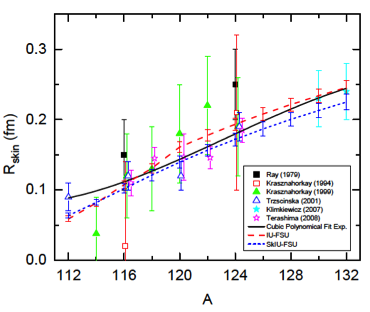
\includegraphics[scale=0.6]{pictures/png/tiniso.png}
\caption{The predictions of the neutron skin thicknesses for tin isotopes from the IU-FSU and SkIU-FSU models after the optimisation with those from different experimental methods \cite{fattoyev}.}
\label{tiniso}
\end{center}
\end{figure}

\subsection{Reaction kinematics}

\indent Schematics of the kinematics of a pion photoproduction reaction are shown in a figure below (Fig. \ref{photorea}). The interacting particles, photon ($\gamma$) and a nucleon (N) have initial four-momenta k and $p_{i}$ respectively. The four-momentum is a combination of particle's energy and its three-momentum: P=(p,E).

\begin{figure}[H]
\begin{center}
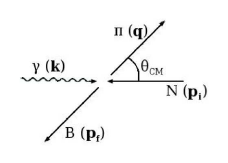
\includegraphics[scale=0.6]{pictures/png/photorea.png}
\caption{Simple diagram of a photoproduction reaction \cite{jo}.}
\label{photorea}
\end{center}
\end{figure}

\indent The Feynman diagrams shown below, illustrate that this reaction can proceed via three possible mechanisms (Fig. \ref{mandelstam}). First diagram, s-channel describes a process where photon and nucleon combine and an intermediate particle (resonance) is formed. In the case of t-channel, one of the interacting particles emits an intermediate particle which is subsequently absorbed by the other interacting particle. U-channel describes the same situation as t-channel with the exception of the final state particles being interchanged.

\begin{figure}[H]
\begin{center}
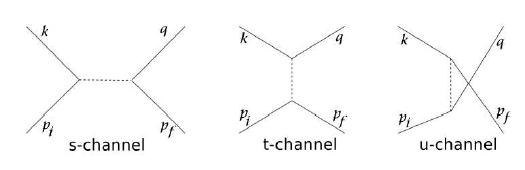
\includegraphics[scale=0.6]{pictures/png/mandelstam.png}
\caption{Feynman diagrams of the s-channel, t-channel and u-channel.}
\label{mandelstam}
\end{center}
\end{figure}

\indent The kinematics of such production reaction can be easily described with the use of Lorentz-invariant Mandelstam variables s, t and u. The mechanisms are commonly referred to as: s-channel, t-channel and u-channel (Fig. \ref{mandelstam}). They are defined in terms of four-momenta as \cite{walker}:

\begin{equation}
s=(k+p_{i})^{2}=(q+p_{f})^{2}
\end{equation}
\begin{equation}
t=(p_{i}-p_{f})^{2}=(k-q)^{2}
\end{equation}
\begin{equation}
u=(p_{i}-p_{f})^{2}=(k-p_{f})^{2}
\end{equation}
s is the square of the energy of the reaction, t is the square of the momentum transfer, while the sum of the squares of the masses of particles is defined as a linear combination of those three variables.

\begin{equation}
s+t+u=\sum\limits m^{2}_{i}
\end{equation}

\indent Only two of the Mandelstam variables are necessary to fully describe the reaction between photon and nucleon. In the relativistic approximation, $mc^{2}<<E$, these variables can be represented as:

\begin{equation}
s=4p^{2}
\end{equation}
\begin{equation}
t=2p^{2}(1-cos\theta)
\end{equation}
\begin{equation}
u=2p^{2}(1+cos\theta)
\end{equation}
where $\theta$ is the pion scattering angle in the centre of mass frame of reference. If $s$ is fixed, t is a linear function of $cos\theta$, and therefore, the scattering functions can be represented completely in terms of $s$ and $cos\theta$ \cite{bertulani}.

\subsection{Reaction cross sections}

\indent For a pion, or any meson, created in a photoproduction process, its angular distribution can be represented by a differential cross section:

\begin{equation}
\frac{d\sigma}{d\Omega}=|A(s,cos\theta)|^{2}
\end{equation}

\indent The probability of the transition from a given initial state $<i|$ to another final state $|f>$ can be represented by a scattering matrix S in the Bjorken Drell notation\cite{bjorken}:

\begin{equation}
S_{fi}=\delta_{}fi-\frac{i}{(2\pi)^{2}}\delta^{4}(q-k+p_{f}-p_{i})\sqrt{\frac{m_{N}^{2}}{4E_{\gamma}E_{\pi}E_{i}E_{f}}}<i|T|f>
\end{equation}
where, $T$ is the transmission matrix relating initial and final states, $m_{N}$ is the mass of a nucleon, and q, k, $p_{i}$, $p_{f}$ are four-momenta of the involved particles. The transition matrix describes the amplitude of the photoproduction process, and can be written as:

\begin{equation}
T=\epsilon_{\mu}J_{\mu}
\end{equation}
where, $\epsilon_{\mu}$ is the photon polarisation vector and $J_{\mu}$ is the electromagnetic current of a nucleon. Then the differential cross section can be defined ac:

\begin{equation}
\frac{d\sigma}{d\Omega}=\frac{q}{k}(\frac{m_{N}}{4\pi W})^{2}\sum |T|
\end{equation}
where, W is the invariant mass of the system.

\indent The electromagnetic current of a nucleon, $J$, as proposed by Chew, Goldberg, Low, Nambu (CGLN), can be written in terms of nucleon spin matrices and meson unit vectors \^q and \^k \cite{chew}:

\begin{equation}
J=\frac{q}{k}\frac{4\pi W}{m_{n}}(i\sigma F_{1}+(\vec{\sigma} \cdot \hat{k})(\vec{\sigma} \times \hat{q})F_{2}+i k(\vec{\sigma} \cdot \hat{q})F_{3}+i k(\vec{\sigma} \cdot \hat{k})F_{4})
\end{equation}
where,
\begin{equation}
\bar{\sigma}=\sigma-(\sigma \cdot \hat{q})\hat{q}
\end{equation}
\begin{equation}
\bar{k}=\hat{k}-(\hat{k} \cdot \hat{q})\hat{q}
\end{equation}
and $F_{1}$, $F_{2}$, $F_{3}$, $F_{4}$, known as CGLN amplitudes, are the structure functions of energy and scattering angle, which can be written in terms of electric and magnetic multipoles and angular momentum through a partial wave expansion FIX THIS FORMULA:

\begin{equation}
F_{1}(\theta)=\sum\limits_{l=0}^{\infty} (lM_{l+}+E_{l+})P'_{l-1}(cos\theta)+((l+1)M_{l-}-E_{l-})P'_{l-1}(cos\theta)
\end{equation}
\begin{equation}
F_{2}(\theta)=\sum\limits_{l=0}^{\infty} ((l+1)M_{l+}+lM_{l-})P'_{l}(cos\theta)
\end{equation}
\begin{equation}
F_{3}(\theta)=\sum\limits_{l=0}^{\infty} (E_{l+}-M_{l+})P"_{l+1}(cos\theta)+((E_{l-}+M_{l-})P"_{l-1}(cos\theta)
\end{equation}
\begin{equation}
F_{4}(\theta)=\sum\limits_{l=0}^{\infty} (M_{l+}-E_{l+}-M_{l}-E_{l-})P"_{l}(cos\theta)
\end{equation}
where, $P'_{l}$ and $P"_{l}$ are derivatives of a Legendre polynomials, $l$ is the relative orbital momentum of a meson, $E_{+/-}$ and $M_{+/-}$ are electric and magnetic transition respectively, and the + or - determine whether the spin of the baryon should be added or subtracted.

\indent The total angular momentum of a nucleon in $\frac{1}{2}$, and the total angular momentum of an incident photon is $L_{\gamma}$. The resulting spin of a resonant state, in order to satisfy the selection rule, has to obey the following relation \cite{krusche}:

\begin{equation}
|L_{\gamma}-\frac{1}{2}|<J_{N*}<|L_{\gamma}+\frac{1}{2}|
\end{equation}
and the parity is given as:

\begin{equation}
\pi_{N*}=\pi_{N}\pi_{\gamma}
\end{equation}
where, $\pi_{N}$, parity of a nucleon, i.e. equal to 1, and $\pi_{\gamma}$, the parity of the photon is equal to:

\begin{equation}
\pi_{\gamma}=(-1)^{L_{\gamma}}
\end{equation}
\begin{equation}
\pi_{\gamma}=(-1)^{L_{\gamma}+1}
\end{equation}
respectively for an electric and magnetic multipoles.

\indent The selection rules for the angular momentum and parity of the resonant state with respect to the outgoing meson are given as:

\begin{equation}
|L_{\pi}-\frac{1}{2}|<J_{N*}<|L_{\pi}+\frac{1}{2}|
\end{equation}
\begin{equation}
\pi_{N*}=\pi_{N}\pi_{\pi}(-1)^{L_{\pi}}=(-1)^{L_{\pi}+1}
\end{equation}
where $\pi_{\pi}$ is -1.

\indent Combining the above equations sets a limit on the spin and parity of the resonance:

\begin{equation}
|L_{\gamma}+/-\frac{1}{2}|<J_{N*}<|L_{\gamma}+/-\frac{1}{2}|
\end{equation}
\begin{equation}
\pi_{N*}=\pi_{N\gamma}=(-1)^{L_{\pi}+1}
\end{equation}

\indent When a cross section is dominated by a single resonance, its quantum numbers are reflected in the angular distribution because the electric multipole $L={L_{\pi}+/-1}$ and magnetic multipole $L={L_{\pi}}$, the spin and parity are related to the angular distribution of mesons for the dependence of the Legendre polynomials in the CGLN amplitudes. Most photoproduction mechanism, however, have more than one multipole contributing to the resonance and in order to tell all the different contributions apart, several channels must be measured.

\indent Isospin, not conserved in the electromagnetic interactions, is conserved however, in the hadronic interactions. The isospin of the initial state, determined from the isospin of the nucleon, is $I_{i}=\frac{1}{2}$ while the contributions from the pion and nucleon's isospins determine the one of the final state, $I_{f}$, which can therefore take values of $\frac{1}{2}$ or $\frac{1}{2}$. The value is determined by the photon which behaves as a linear combination of isoscalar ($I_{s}$) which conserves the isospin and isovector ($I_{v}$) which can change the isospin by one, components. The whole system can be then described by the three isospin amplitudes \cite{nagl}:

\begin{equation}
A^{0}=<\frac{1}{2},I_{3}|I_{s}|\frac{1}{2},I_{3}>
\end{equation}
for the isoscalar electromagnetic current
\begin{equation}
A^{1}=<\frac{1}{2},I_{3}|I_{v}|\frac{1}{2},I_{3}>
\end{equation}
\begin{equation}
A^{3}=<\frac{3}{2},I_{3}|I_{v}|\frac{1}{2},I_{3}>
\end{equation}
while for the isovector electromagnetic current, the amplitudes are written as \cite{davidson}:

\begin{equation}
A^{+}=\frac{A^{1}+2A^{3}}{3}
\end{equation}
\begin{equation}
A^{-}=\frac{A^{1}-A^{3}}{3}
\end{equation}

\indent In terms of isospin amplitudes, the physical amplitudes for pion photo production are written as:

\begin{equation}
A(p\gamma \rightarrow n\pi^{0})=<p\pi^{0}|I|p\gamma>=(A^{0}+A^{+})
\end{equation}
\begin{equation}
A(n\gamma \rightarrow n\pi^{0})=<n\pi^{0}|I|n\gamma>=(A^{+}+A^{0})
\end{equation}
\begin{equation}
A(p\gamma \rightarrow n\pi^{+})=<n\pi^{+}|I|p\gamma>=\sqrt{2}(A^{0}+A^{-})
\end{equation}
\begin{equation}
A(n\gamma \rightarrow p\pi^{-})=<p\pi^{-}|I|n\gamma>=\sqrt{2}(A^{0}-A^{-})
\end{equation}
The above set of equations allows for the separation of the amplitudes for individual photoproduction reactions provided that the measurements on both proton and neutron targets are carried out.

\subsection{Partial Wave Analyses}

\indent In order to extract information on the masses, widths and amplitudes from the experimental data, different reaction models have been developed and used. The most common approach involves separation of background and resonant terms of a transition matrix.

\indent Considering a reaction of the form $A\rightarrow B\rightarrow C$, where $A$ is the initial state of the nucleon-photon system,$B$ is the intermediate resonant state and $C$ is the final state of the nucleon-meson system, the photoproduction process can be described with a below Hamiltonian:

\begin{equation}
H=H_{0}+V_{bg}+V_{R}(E)
\end{equation}
where, $H_{0}$ is a free Hamiltonian expressing the total kinetic energy of the interacting particles, $V_{bg}$ is the potential due to the background created by the non-resonant contributions to the reaction, and $V_{R}$ is potential due to resonant term.

\indent The transmission matrix for the process is given as:

\begin{equation}
T_{AC}=V_{AC}+\sum\limits_{B}V_{AB}g_{B}(E)T_{BC}(E)
\end{equation}
where, $g_{B}$ is the propagator of the channel B of the reaction, and $\sum\limits_{B}$ sums all the possible channels of the reaction $A\rightarrow C$ via $B$. Alternatively, the transmission matrix can be split into the background and resonant terms what allows for independent calculations of for the background and resonant contributions.

\begin{equation}
T_{AC}=t_{bg}^{AC}+t_{R}^{AC}(E)
\end{equation}

\indent Partial wave analyses (PWA) are methods that allow for decomposition of the background and resonant terms of the transmission matrix into a number of partial waves of defined multipoles and momentum. Generally, the resonant terms are modelled with a Breit-Wigner form while the background is described with Born terms and vector-meson contributions. The extractions of the parameters from the analysis is done with a two-stage procedure of fitting the experimental data. The most commonly used for the pion photoproduction PWAs are MAID, developed at the University of Mainz \cite{maid}, and SAID written by the CNS Data Analysis Centre at George Washington University \cite{said}.

\indent MAID is a unitary isobar model which describes the transmission matrix through a single $\pi N$ channel \cite {drechsel}:

\begin{equation}
T_{\gamma\pi}=V_{\gamma\pi}(E)+V_{\gamma\pi}(E)g_{B}(0)T_{\pi N}(E)
\end{equation}
where, $V_{\gamma\pi}$ is the transition potential of the $\gamma N\rightarrow \pi N$ reaction, $T_{\pi N}$ and $g_{0}$ are the scattering matrix and the free propagator of the $\pi N$ interaction respectively.

\indent The scattering matrix and the transition potential can be broken down to its constituents background and resonant terms and those can be expanded as partial waves. The resonances included in MAID, classified as 4* by the Particle Data Group (PDA) \cite{pda}, are all only up to $2GeV$.

\indent In the methods developed for SAID, there are no assumptions about resonances and channels included in the analysis framework. The transmission matrix, defined for the following three channels: $\gamma N$, $\pi N$ and $\pi \Delta$ (covering all open channels), can be written as \cite{arndt}:

\begin{equation}
T_{\gamma\pi}=A_{1}(1+iT_{\pi N})+A_{R}T_{\pi N,\pi N}
\end{equation}
where $A_{R}$ parametrises the multipole amplitudes of the resonant terms, and $A_{1}$ parametrises background.

\begin{equation}
A_{R}=\frac{m_{\pi}}{q}[\frac{k}{q}]^{l}\sum\limits_{n=0}^{N}p_{n}[\frac{E_{\pi}}{m_{\pi}}]
\end{equation}
\begin{equation}
E_{\pi}=\frac{s-(m_{\pi}+M)^{2}}{2M}=E_{\gamma}-m_{\pi}(1+\frac{m_{\pi}}{2M})
\end{equation}
where $E_{\pi}$ is the pion kinetic energy in the lab frame for the $\pi N\rightarrow \gamma N$, s is the square of the centre of mass energy, $M$ is the mass of the nucleon and $E_{\gamma}$ is the photon lab energy for $\gamma N \rightarrow \pi N$, and $p_{n}$ is a free parameter determined in the fit to the experimental data.

\begin{equation}
A_{1}=A_{B}+A_{Q}
\end{equation}
where, $A_{B}$ is a partial wave of a pseudoscalar Born amplitude, and $A_{Q}$ is a Legendre function.

\indent Detailed explanation of MAID and SAID can be found in \cite{maid} and \cite{said, arndt}.

\section{Nuclear Matter Distribution}

\indent ?

\subsection{The nuclear Equation of State}

\indent By definition, the equation of state (EOS) is a function of density ($\rho$) and isospin asymmetry ($\alpha$) and it's expressed as the energy (E) per nucleon in the infinite nuclear matter, $\frac{E}{A} (\rho,\alpha)$ where $\alpha$ is expressed as:

\begin{equation}
\alpha=\frac{N-Z}{A}
\end{equation}
where $N$ is the number of neutrons,$Z$ is the number of protons and $A$ is the atomic mass number.

\indent The Bethe-Weizsaecker mass formula, more commonly known as semi-empirical mass formula, based on the theory of the liquid drop model, have been first proposed in 1935 to explain the various properties of an atomic nucleus. According to the formula, the binding energy, $E_{B}$ can be approximated as:

\begin{equation}
E_{B}=a_{V}A^{3}-a_{s}A^{\frac{2}{3}}+a_{C}\frac{Z^{2}}{A^{\frac{1}{3}}}-a_{A}\frac{(A-2Z)^{2}}{A}-\delta(A,Z)
\end{equation}
where, $a_{V}$ is the volume coefficient (based on the strong force), $a_{S}$, also based on the strong force, is a surface term which provides a correction to the volume term, $a_{C}$ is the Coulomb or electrostatic term which introduces a correction due to electrostatic repulsion. $a_{A}$ is the assymetry coefficient arises from the Pauli exclusion principle, and accounts for the imbalances between numbers of proton and neutrons in a nucleus. The pairing term $\delta(A,Z)$ covers the effects of spin-coupling \cite{bertulani}.

\indent

\section{Previous Measurements}

\indent Neutron skin measurements have been performed with strongly interacting probes before. The obtained data were strongly affected by many-body strong interaction effects that made the analysis and interpretation of the results ambiguous and difficult to draw binding conclusions from. The experiment involving proton scattering data fitted with different neutron skin thicknesses concluded with data being unable to determine the size or even the existence of the neutron skin \cite{piek}.

\indent The measurement of parity violation in electron scattering provides an independent probe of neutron densities because the weak charge of the neutron is much larger than that of proton. The interpretation of such results is model-independent and unaffected by the uncertainties of strong interactions. The polarised electrons have been used as a probe of neutron distribution in the $^{208}$Pb Radius Experiment (PREX). It made use of parity violation to accurately determine the neutron radius of the lead nucleus. The first measurement of the parity-violating asymmetry, $A_{PV}$ in the elastic scattering of polarised electrons from $^{208}$Pb reports the thickness of neutron skin of $\Delta R = 0.33_{-0.18}^{+0.16}$fm, and therefore provides the first electroweak observation of the neutron skin. \cite{prex}.

\indent The experiment investigating nuclear periphery at Low Energy Antiproton Ring (LEAR) at CERN allowed for an estimate of the relation between the symmetry parameter and neutron skin. 26 isotopes with mass numbers in a range of 40-238 have been studied. Antiprotons were chosen as a probe for the experiment since the antiproton-nucleus interactions are very strong and even a small overlap between their wave functions leads to the annihilation of the antiproton with one of the peripheral nucleons resulting in a final state nucleus with either proton or neutron number lower by one unit compared to the initial state. If both products are radioactive nuclear spectroscopy can be employed to determine their relative yields which are directly related to the proton and neutron densities at the annihilation site. The experimental results are presented in (Fig. \ref{antiproton}); analysis of the data indicated that neutrons are distributed in a form of a halo rather than a skin \cite{trzcina}. However, as the antiprotons are absorbed only in the surface of the nucleus the systematics in such measurements are somewhat controversial.

\begin{figure}[H]
\begin{center}
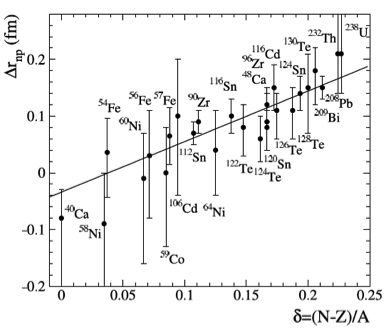
\includegraphics[scale=0.6]{pictures/png/antiproton.png}
\caption{Difference between the r.m.s. radii of the neutron and proton distributions ($\Delta r_{np}$) against the symmetry parameter $\delta$. Picture taken from the reference \cite{trzcina}.}
\label{antiproton}
\end{center}
\end{figure}



%now here you can refer to the first section like, see section \ref{sec1}......


\setcounter{equation}{0}
%\setcounter{figure}{0}
%\setcounter{table}{0}

\chapter{Experimental details}

\section{Overview}

\indent The experiment has been performed in the A2 hall of MAMI facility at the Johannes Gutenberg Universitaet in Mainz, Germany in October 2012 over the course of 21 days.

\indent The key element of the MAMI installation is the Mainzer Mikrotron; it provides a 100\% duty factor electron beam that can be directed to any one of the four experimental halls. The photon beam utilized in the experiment was produced by directing the electron beam onto a thin metallic radiator creating bremsstrahlung radiation. The Glasgow Photon Tagger analyses the recoiling electrons from the bremsstrahlung process and provides information on the energy of the photons. The tagger comprises of a large dipole magnet with an highly segmented detector apparatus near its focal plane. The tin target, located in the center of the Crystal Ball (CB), has been exposed to this bremsstrahlung photon. The products of the resulting photoreactions is then detected with the A2 segmented detectors. Since neutral pions have a very short lifetime, of the order of ~10$^{-18}$s it is not possible to detect them directly. Instead, the products of their dominant decay, two photons, are detected in the apparatus and the pion's 4 momentum is reconstructed from this information. A schematic picture of the MAMI facility is presented In Fig. \ref{a2hallsetup}.

\begin{figure}[H]
\begin{center}
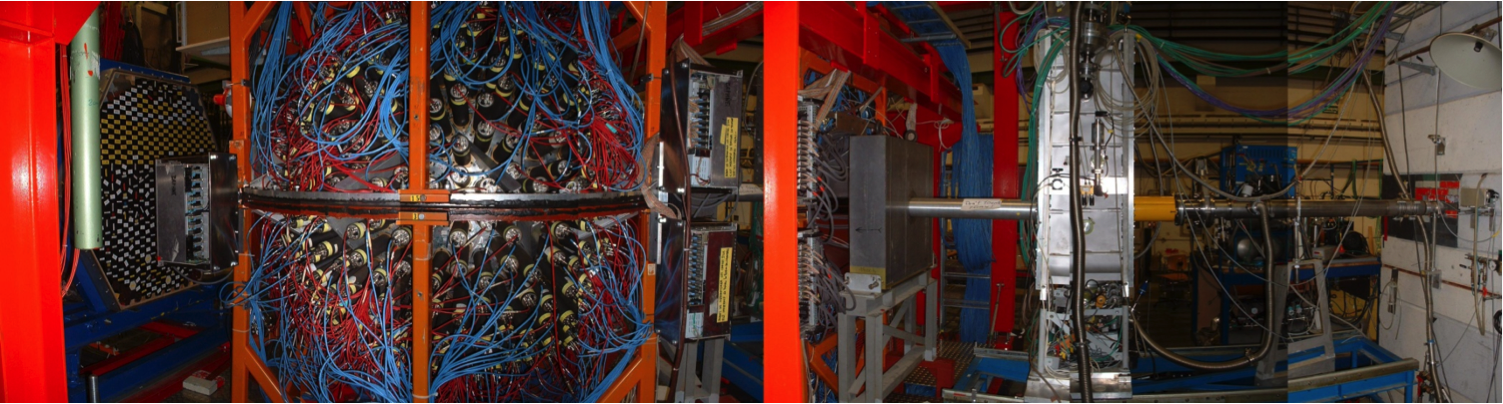
\includegraphics[scale=0.55]{pictures/png/a2hallsetup.png}
\caption{A diagram illustrating the experiential setup in the A2 hall at MAMI.}
\label{a2hallsetup}
\end{center}
\end{figure}

In addition to the CB and TAPS detectors we also used information from  the Edinburgh Particle Identification Detector (PID), which provides information about charged particles detected in CB, and the Multi Wire Proportional Chambers (MWPC), which provides identification of charged particles and tracking information. The details of all the detectors as well as the MAMI facility itself are presented in the following sections.

\section{Mainzer Mikrotron}

\indent The Mainz Microtron (MAMI) is a continuous wave electron accelerator. It is located at the Institut fuer Kernphysik at Johannes Gutenberg Universitaet in Mainz, Germany. MAMI operates since 1979 and in the interim period has been upgraded three times, achieving successively higher electron beam energies and intensities. The most recent upgrade, to MAMI-C, provides an  electron beam energy up to 1.6GeV with an 80\% helicity polarization and a beam current of over 20$\mu$A (unpolarized electron beams can reach up to 100$\mu A$).

\indent The MAMI facility operates using a racetrack microtron design.  In this a beam of electrons is accelerated by a series of radio frequency LINAC (linear accelerator) sections and recirculated through the LINACs using a magnetic field. Each time the beam passes through the LINAC its orbit through the magnetic field changes, with higher energy electrons taking wider paths through the magnetic field. These paths are finely tuned such that the electrons always pass through the linac in time with the correct radiofrequency (rf) electric field applied to the LINACs.  The design of the early stages of the MAMI RTM employs two homogeneous semicircular magnets and a small linear accelerator (LINAC) placed between them (Fig. \ref{microtronplot}).
Repeated passes through LINAC ensure that high beam energy can be achieved even if the acceleration with each pass is relatively small. The first microtron has been constructed at the National Research Council of Canada in 1947, according to the design of V. I. Veksler, where the electrons, accelerated along circular paths, reached energies of up to 4.6MeV \cite{dehn}. Ever since that first design the idea of a microtron has been worked upon to reach higher electron energies. The concept of a  racetrack microtron (RTM) has been proposed already in 1945 but the first RTM was constructed only in 1961 and provided electron beams of energies up to 12~MeV. 
\begin{figure}[H]
\begin{center}
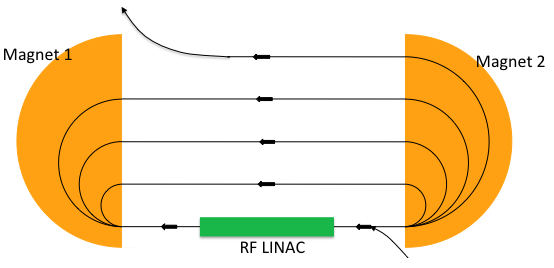
\includegraphics[scale=0.55]{pictures/png/rfm.png}
\caption{Schematics of a simple microtron.}
\label{microtronplot}
\end{center}
\end{figure}

In 1979 a RTM was first used successfully at the MAMI facility, producing an electron beam of 14MeV (MAMI-A1). Subsequent upgrade (MAMI-A2) introduced another RTM to the design and allowed for beam energies up to 180MeV in 1983. The need for even higher beam energies inspired yet another upgrade (MAMI B), and in 1990 with the addition of another RTM it was possible to achieve energies of up to 855MeV. However, quickly advancing research in the fields of nuclear and particle physics required even higher energies. The design allowing for beam energies of 1.5GeV however, could not employ another RTM based on the dipole magnet design; the magnets required for achieving such energies would have to weight 2500 tons each which was neither financially nor spatially feasible; for comparison, magnets in the MAMI B design weigh only 450 tons. The issue has been bypassed by adding a harmonic double-sided microtron (HDSM). In this concept, rather than using two magnets bending the beam by 180$^{\circ}$, have been used four 90$^{\circ}$ magnets and two accelerating sections (Fig. \ref{mamic}). 

\begin{figure}[H]
\begin{center}
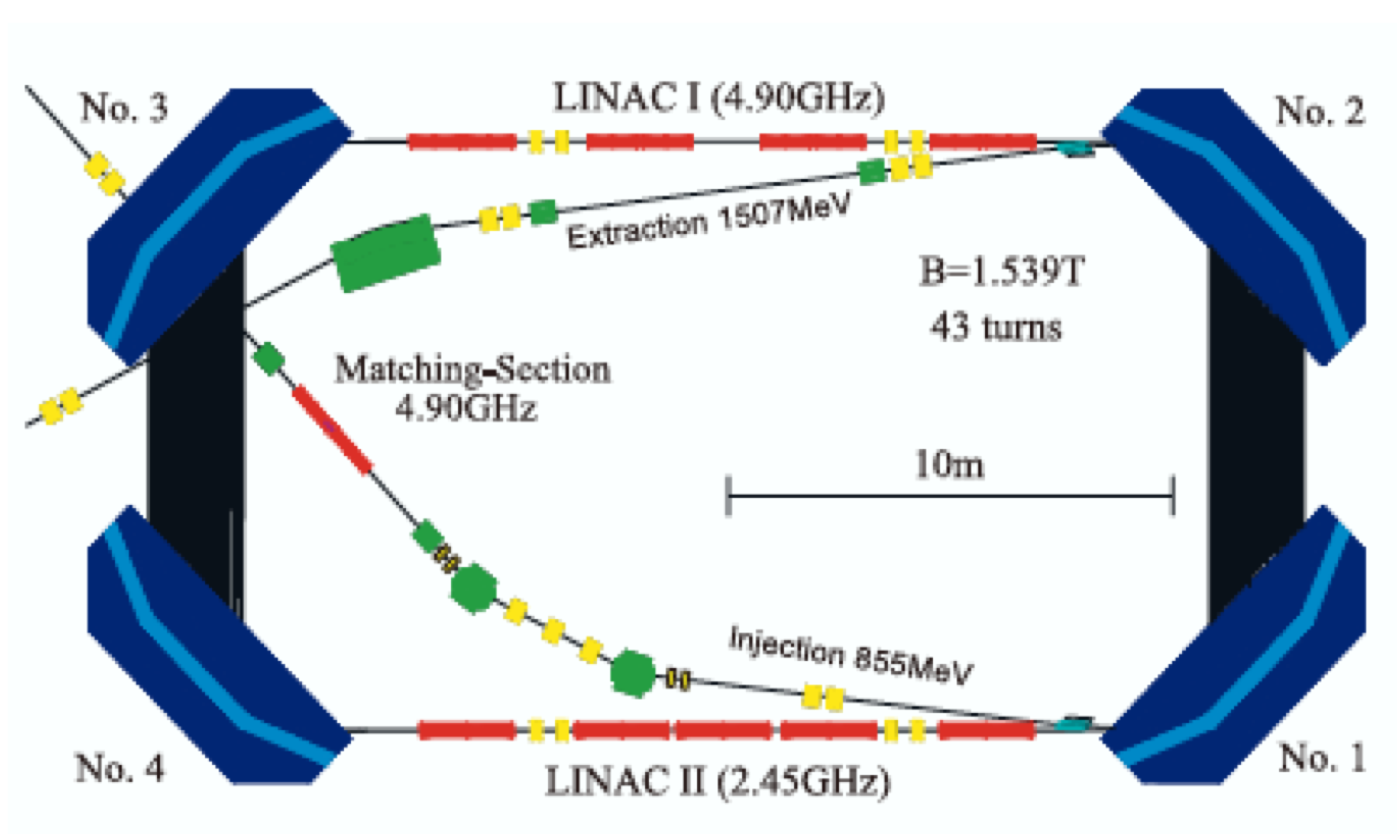
\includegraphics[scale=0.25]{pictures/png/HDSM.png}
\caption{Schematic picture of a harmonic double-sided microtron for MAMI C.}
\label{mamic}
\end{center}
\end{figure}

This design allowed for the production of a 1.508GeV electron beam in December 2006, and energy as high as 1.604GeV has been reached in 2009.

\begin{figure}[H]
\begin{center}
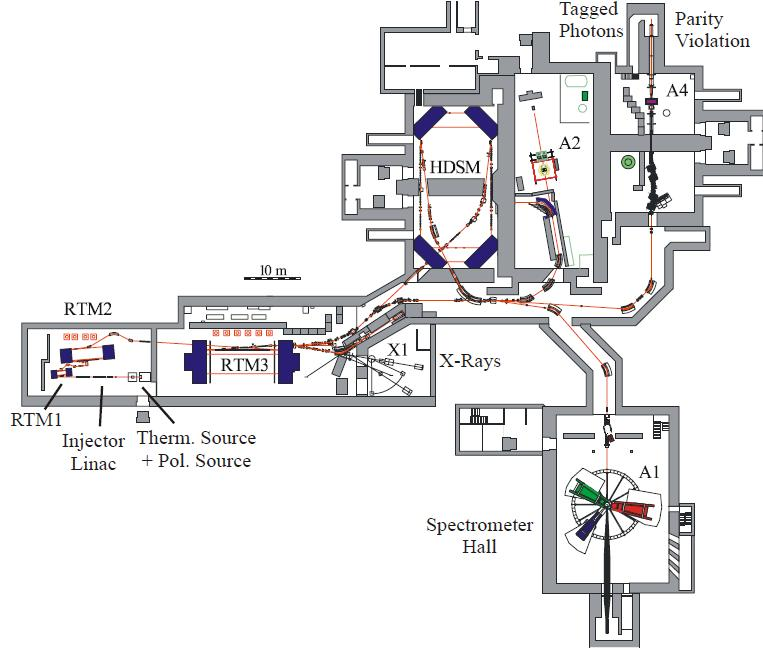
\includegraphics[scale=0.5]{pictures/jpg/mamifloor.jpg}
\caption{Floor plan of the MAMI facility.}
\label{mamifloor}
\end{center}
\end{figure}

\section{Glasgow Photon Tagger}

\indent The experiment has been performed in the A2 hall of MAMI (Fig .\ref{mamifloor}), which houses the installation dedicated to the studies of reactions between high-energy photons with different atomic nuclei. The photon beam used in this experiment has been produced through the electrons ejected from RTM3 which were directed into the A2 hall into a thin, 10$\mu$m thick, copper radiator. The 855MeV electrons can interact in the electrostatic field of the copper nuclei and radiate photons; the energy of these bremsstrahlung photons can be calculated from:

\begin{equation}
E_{\gamma}=E_{0}-E_{e}
\end{equation}

where $E_{0}$ is the initial beam energy and $E_{e}$ is the energy of the scattered electrons. This equation neglects the energy loss to the recoiling copper nuclei, however, the mass of the copper nucleus is high enough to assume that only negligible amount of kinetic energy has been transferred.

\begin{figure}[H]
\begin{center}
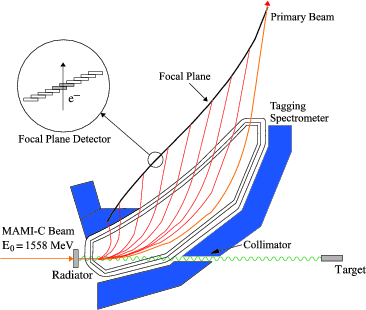
\includegraphics[scale=0.8]{pictures/png/GlaTagger.png}
\caption{Schematic picture of the Glasgow Photon Tagger \cite{marcu}.}
\label{gpt}
\end{center}
\end{figure}

\indent The Glasgow Photon Tagger (GPT) is a large momentum acceptance spectrometer. Electrons, after passing through the radiator, first enter the magnetic field of a quadrupole magnet, which focuses them vertically. After, the resulting electrons pass through a dipole magnet which disperses them horizontally according to their energy. For example, the lower energy electrons associated with the production of higher energy photons are bent more significantly by the field compared to the higher energy electrons. The momentum of the bremsstrahlung electrons is analyzed in the Glasgow Photon Tagger (Fig. \ref{gpt}). By identifying the path of the electron in the field and correlating the timing of the electron with the subsequent photonuclear reaction in the target then the photons can be characterized event-by-event. This is referred to as a tagged photon beam. Electrons that have radiated bremsstrahlung photons are directed onto a segmented focal plane detector. The electrons that haven't radiated any photons follow a curved path into a beam dump.

\indent The Focal Plane (FP) detector consists of 353 plastic scintillator detectors wrapped in a double-sided, aluminized Mylar \cite{sjhall}. Each of these scintillators is 80mm long and 2mm thick with a varying width of 9-32 mm. The detector width decreases along the focal plane in order to keep the energy resolution constant. The scintillators overlap by more than a half-width (Fig 3.2) which allows for electron detection by coincident signals in two adjacent detectors. The size of this overlap fixes the achievable energy resolution, which ranges from 2-8MeV with an average of 4MeV, depending on the beam energy \cite{mcgeorge}; the coincidence condition also allows for significant reduction of the low energy background in the detector.

\indent Each scintillator is connected to an R1635 Hamamatsu photomultiplier tube (PMT), which are shielded from the magnetic field by 0.7mm thick steel plates and an individual sheath of $\mu$-metal. The high segmentation of the array allows for the tagging of high-flux photon beams. When used with the 1.508GeV electron beam, the tagger can operate at a rate of up to 10$^{8}$ s$^{-1}$ flux photons in the energy range of 0.08-1.401GeV. The maximum rate is determined by the operating limit of the individual PMTs being 1MHz per channel, limit used in order to avoid unnecessary reduction of their operating lifetime. The bremsstrahlung photons pass the magnetic field of the GPT unaffected and exit into the experimental hall through a channel bored into the dipole magnet.

\indent In order to ensure the small size of the beam spot on the target a 3mm collimator is employed near to the exit of this bored channel. Employing a collimator produces a more well defined beam spot on the target, but also reduces the photon flux.  Without collimation, the photon flux incident upon the target would be related more directly to the number of hits in the FP detector. To determine the exact luminosity of the photon beam, tagging efficiency measurements have to be made where a 100\% efficient lead glass detector is placed in the beamline.  This efficiency correction is applied individually to each detector channel in the focal-plane detector, as the efficiency depends on the opening angle of the gamma beam, which depends on the gamma (or electron) energy. The tagging efficiency is defined as:

\begin{equation}
\epsilon_{tagg}=\frac{N_{\gamma}}{N_{e}}
\end{equation}

\indent where $N_{\gamma}$ is the number of photons passing through the collimator and registered by the lead glass detector, and $N_{e}$ is the number of hits in the FP detector. During the tagging efficiency measurement, carried out as separate runs during the experiment, a lead glass detector is placed in the path of the collimated beam. The beam intensity employed in this measurement is lower than that used in the actual experiment in order to protect the lead glass detector from the potential radiation damage and to reduce the number of multiple hits in the FP detector.

\section{Crystal Ball}

\indent The Crystal Ball (CB) has been constructed and used in various experiments long before  being  installed  at  MAMI.  First  used  in the 1970s  for colliding  beam experiments at the SLAC facility to obtain first accurate measurements of $\frac{J}{\psi}$ \cite {oreglia}. Later it has been used at DESY and in Brookhaven National Laboratory and arrived in its current home, the A2 hall at MAMI only in 2002. The CB is an highly segmented calorimeter, it consists of 672 sodium iodide (NaI) crystals, each in a shape of truncated triangular pyramid, and arranged into a shape of a 20 sided polyhedron (Fig. \ref{naigeom}).

\begin{figure}[H]
\begin{center}
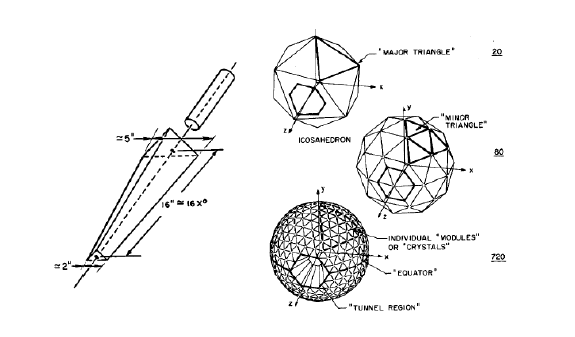
\includegraphics[scale=0.7]{pictures/png/naigeom.png}
\caption{NaI crystal and CB geometry \cite{a2mami}.}
\label{naigeom}
\end{center}
\end{figure}

\indent Having  been  designed  for  the  colliding  beam  experiments,  the  plan  had  to accommodate  the  beamline  running  across  and  through the  center  of  the  CB. Because of that the section corresponding to 24 crystals on opposite poles of the sphere  has  been  cleared  making  room  for  the  beamline  components.  The remaining crystals have been grouped into two, hermetically sealed hemispheres; the isolation of the crystals from the outside environment was essential because NaI is an highly hygroscopic and it degenerates when exposed to the air moisture.

\indent The outer and inner radii of the CB are 66cm and 25.3cm respectively. The two hemispheres are enclosed within a 1.5mm thick steel casing and the width of the gap between them, the equator region, is 0.8cm thick and consists of two 1.6mm thick steel plates and an adjustable air gap, usually set to 5mm. Such design allows for the coverage close to complete angular range, ~94\% of 4$\pi$.

\indent The of the 20 faces (major triangle) of the CB polyhedron is segmented into 4 smaller triangles (minor triangle)  which  are in turn divided into 9 segments corresponding to individual NaI crystals (Fig. \ref{naigeom}). Each crystal, 40.6cm long with the sides of the inner and outer faces being 5.1cm and 12.7cm respectively, is optically shielded with a reflector paper and aluminized Mylar, and connected to the 5.1cm diameter SRC L50 B01 PMT, chosen for a good linear response over a wide range of energies. These are mounted outside the CB and scintillation light is fed into them through a 5cm air gap and a thick glass window, separating the NaI crystals from the PMTs. This set up constitutes part of the hermetic design helping to maintain isolated environment for the sodium iodide crystals. During the experiment photons produced in the reactions inside the CB trigger an electromagnetic shower which deposits energy in the NaI crystals. This system allows for good energy resolution across a wide range of energies. The amount of deposited energy and the number of crystals hit depend on the reaction studied; the  information  about  the  nature  of  the  particles  detected  in  the  CB  are recovered from the analysis of the hits in the NaI clusters; the basic detection properties  of  the  CB  are  summarized  in  the  below  table \cite {starostin}.
 
\begin{table}[ht]
\caption{Crystal Ball Detection Parameters}
\centering
\begin{tabular}{c c c}
\hline\hline
Energy Photon Resolution & &  \\
 & $\frac{\sigma}{E}$ & $\sim \frac{1.7\%}{E(GeV^{0.4})}$ \\
\hline
Angular Resolution & & \\
 & azimuthal: & $\sim \frac{2^{\circ}}{sin\theta}$ \\
 & polar: & $\sim 2-3^{\circ}$ \\
\hline
Angular Coverage & & \\
 & azimuthal: & 0 - 360$^{\circ}$ \\
 & polar: & 20 - 160$^{\circ}$ \\
\hline
Time resolution & & \\
 & & $\sigma \sim 2ns$ \\
\hline\hline
\end{tabular}
\label{table_cbparam}
\end{table} 
 

\section{Multi Wire Proportional Chambers}

\indent Inside the tunnel region in the Crystal Ball another detector by the name of Multi Wire Proportional Chambers (MWPCs) is located. The task of this apparatus is to retrieve  information  about  charged particles and it follows  the  same design  as the  one originally used in DAPHNE \cite{audit}.

\indent Each of the two MWPCs is built up of three layers; internal and external stripes acting as cathodes and a middle layer of wires as the anode (Fig. \ref{mwpc}). The cylindrical  cathodes  are  made  from  1mm  thick  rohacell  laminated  with aluminum stripes, 4mm wide and  0.1$\mu$m thick, spaced 0.5mm apart. The stripes are  wound  helically  at  45$^{\circ}$  with  respect  to  the  anode  wires, at  opposite directions.  The  anode  is  made  up  of  20$\mu$m  Tungsten  wires  2mm  apart placed parallel to the beam direction. The chambers are filled with a gas mixture of argon(79.5\%), ethane (30\%) and freon (0.5\%).

\begin{figure}[H]
\begin{center}
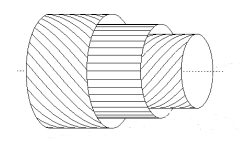
\includegraphics[scale=1.0]{pictures/png/mwpc.png}
\caption{Diagram of MWPC showing the positions of anode wires and cathodes stripes \cite{jalbert}.}
\label{mwpc}
\end{center}
\end{figure}


\indent Correlating  the  hits  in  both  the cathode  stripes  and  the  anode  wires  will determine the tracks for charged particles. In the case of neutral particles experiments use the information provided by the MWPCs to determine the position of the target inside the CB. This information is extracted from the linear fit to the polar angle and z-position of the hits registered in both chambers to obtain the azimuthal and theta and angles for each track. Then the trajectories of multiple tracks are analyzed to find their intersection, and therefore obtain the position of the target. The design of the chambers allows this detector for full 360$\deg$ coverage of the azimuthal angle with polar coverage that ranges between 21$^{\circ}$ and 159$^{\circ}$; the characteristics of the MWPC chambers are summarized in the below table.

\begin{table}[ht]
\caption{MWPC parameters}
\centering
\begin{tabular}{c c c}
\hline\hline
Angular Resolution & & \\
 & azimuthal: & $\sim 1.8^{\deg}$ \\
 & polar: & 2$^{\deg}$ \\
\hline
Angular Coverage & & \\
 & azimuthal: & 0 - 360$^{\circ}$ \\
 & polar: & 21 - 159$^{\circ}$ \\
\hline\hline
\end{tabular}
\label{table_mwpc}
\end{table} 

\section{Particle Identification Detector}

\indent The Edinburgh Particle Identification Detector (PID) is located inside the Crystal Ball and it is surrounded by the MWPCs. It is a $\frac{dE}{dx}$ detector and, together with the CB apparatus, it provides information about charged particles.

\indent PID consists of 24 EJ204 plastic scintillators arranged in cylindrical shape. Each scintillator strip is 500mm long and 4mm thick, and, in order to minimize the gaps between adjacent scintillators, the design demanded that they should have a right-angle trapezium cross-section. Each strip is wrapped in an aluminized Mylar foil in order to  optically  isolate  the scintillation  light.  The  scintillators  are  connected  to different PhotoMultipliers (PMT), Hamamatsu R1635 and E1761-04 via perspex light guides. An aluminum ring with 24 holes supports the construction  where the PMTs are positioned in order to match the arrangement of  the  scintillator  strips (Fig. \ref{pid}).  The  entire detector is wrapped in a black Tedlar foil to ensure the lightproof of the detector.

\begin{figure}[H]
\begin{center}
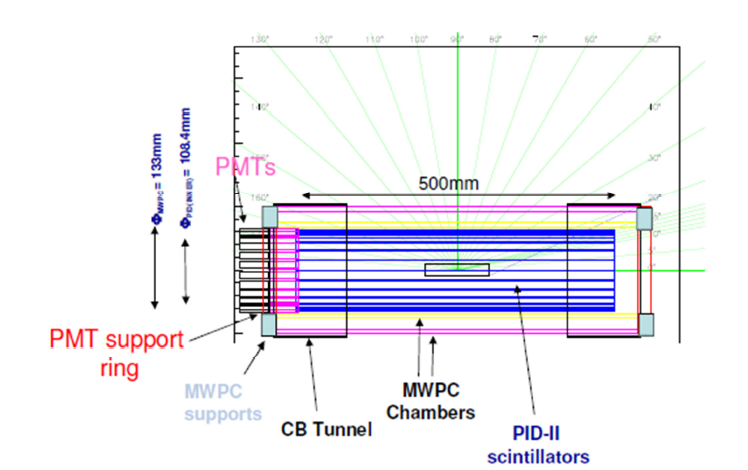
\includegraphics[scale=0.5]{pictures/png/pidschematics.png}
\caption{PID schematics.}
\label{pid}
\end{center}
\end{figure}

\indent The design of the PID allows for the full coverage of the azimuthal angle and for the coverage from 20$^{\circ}$ to 160$^{\circ}$ of the polar angle. This coverage matches exactly the parameters of the CB. When  a  charged  particle  passes  through  the  scintillator  it  deposits  a fraction of its energy while the rest of its energy will be detected in the Crystal Ball. The identity  of  such  particle  is  determined  by  correlating  the  events  from  both detectors while enforcing that the hit in the CB is within 15$^{\circ}$ from the center of the PID scintillator (azimuthal angle). When plotting the energy deposited in the PID against the energy registered in the CB on a two-dimensional plot a characteristical shape is obtained (Fig. \ref{banana}). The proton and pion distribution are easily identifiable in such a plot.

\begin{figure}[H]
\begin{center}
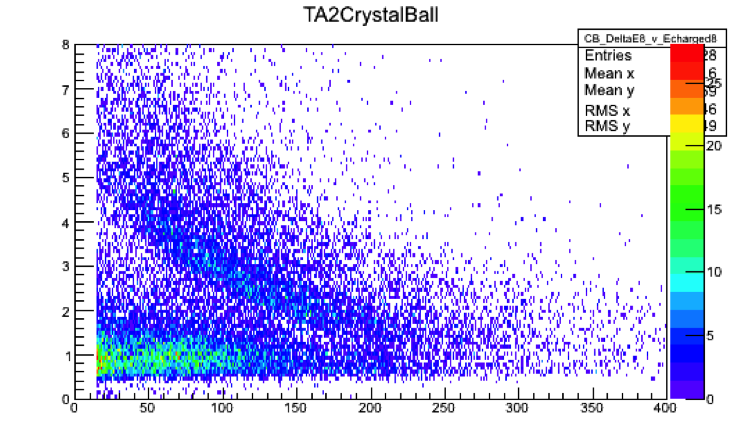
\includegraphics[scale=0.8]{pictures/png/banana.png}
\caption{$\Delta$E-E plots of PID and CB energy deposits.}
\label{banana}
\end{center}
\end{figure}

\section{TAPS}

\indent The Crystal Ball detector has been designed for colliding beam experiments: For this reason the detector  doesn't  cover  $\sim 20^{\circ}$ in the polar  angle  range  for both the  backward  and  the forward direction. In order to fill this gap,  another detector had to be added to the system: the TAPS detector. In MAMI,  the  CB  is  used  for fixed  target  experiments. This kind of experiments are characterized by the fact that the reaction products are Lorentz boosted forward. For this reason it is crucial for many experiments that the additional TAPS detector  covering  those  missing  forward  20  degrees has  been  mounted \cite{novotny}.

\indent TAPS is located 1.5m downstream from the reaction vertex. It is a segmented calorimeter detector made from 385 hexagonal BaF2 crystals (Fig. \ref{taps}). Each crystal is  25cm long,  wrapped in  8  layers  of 38um thick  UV-reflecting PTFE (Teflon) foil and a single layer of 15$\mu$m thick aluminum foil in order to assure light proofing. The cylindrical end part of each crystal is connected to an Hamamatsu R2059 PMT through silicone glue.

\indent The barium fluoride crystals, even though have much lower scintillation output than the NaI crystals used in CB, have higher density (4.89g/cm3) and larger atomic number. These characteristics provide just as good detection efficiency. Another key property of the BaF2 crystals over other materials is their fast timing resolution ($\sim 0.6ns$), which makes the detector ideal for identifying particles through time of flight (TOF) methods \cite{novotny}.


\begin{figure}[H]
\begin{center}
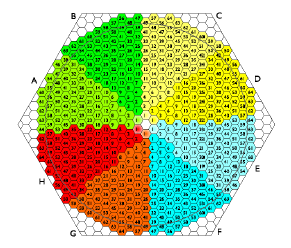
\includegraphics[scale=1.4]{pictures/png/taps.png}
\caption{Diagram of the BaF2 crystals arrangement in TAPS. Different colors represent sectors that can be used in the trigger if required.}
\label{taps}
\end{center}
\end{figure} 

\indent Directly  in  front  of  TAPS,  there  is  an  array  of  5mm  thick  NE102A  plastic scintillators which constitute the TAPS Veto detector. The output from this detector is collected by optic fibers in Valvo XP2972 phototubes. This addition to TAPS allows the discrimination between neutral and charged particles by correlating events from TAPS Veto and TAPS. This allows charged particles to be identified as a function of their energy and energy deposition.

\indent As mentioned before, a parallel method used by TAPS in order to identify particles is through the time of flight of the particles. By measuring  the  time used by a  particle to travel  from  the  target  to the TAPS detector one can discriminate between higher mass particles (like protons and neutrons) and particles traveling at or almost at the speed of light like photons and electrons.

\indent A different method of particle identification, the pulse shape analysis, exploits the fact  that  BaF2  crystals  have  fast  (~0.6ns)  and  slow  (~620ns)  decaying components. Each particle type leaves its own particular imprint on slow and fast components and by comparing the ratios of energy deposited in both, it is possible to improve the particle identification process.

\section{Targets}

\indent A previously performed experiment of coherent $\pi^{0}$ photoproduction on $^{208}$Pb target confirmed the existence of the neutron skin. However, in order to confirm the conclusions of that measurement it was desirable to repeat the experiment with another  heavy  nuclei.  Furthermore,  it  has  been shown  that establishing the evolution of the neutron skin  along  an isotopic  chain  promise  better  results  to  put  tighter constraints on the parameters of the neutron rich matter equation of state \cite{centelles}.

\indent The targets used in this experiment were three isotopes of tin ($^{116}$Sn, $^{120}$Sn and $^{124}$Sn); chosen because of its stability, and because these elements easy of availability. Theoretical  calculations  predict  a change of  ~0.05  to  0.15fm  in  the neutron  skin thickness when going across the isotopic chain of tin from $^{116}$Sn to $^{124}$Sn (Fig. \ref{isochain}) \cite{liewen}. Measuring the skin thickness across the  isotopic  chain  cancels  out  any systematic error,  and  therefore,  allows  to accurately measure the changes predicted by the models.


\begin{figure}[H]
\begin{center}
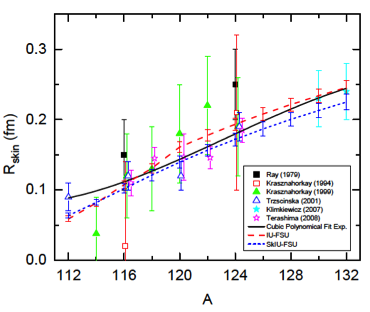
\includegraphics[scale=0.8]{pictures/png/tiniso.png}
\caption{Predictions of neutron skin thickness for tin isotopes from the IU-FSU and SkIU-FSU models.}
\label{isochain}
\end{center}
\end{figure} 

\indent The targets were secured in a target holder and placed inside a PVC tube at the center of detectors. The details of the targets are given in the below table.

\begin{table}[ht]
\caption{Tin targets}
\centering
\begin{tabular}{c c c c c}
\hline\hline
Isotope & mass(MeV) & thickness(mm)  \\
\hline
$^{116}Sn$ & 107961.738 & 1.0 \\
\hline
$^{120}Sn$ & 111688.180 & 0.5 \\
\hline
$^{124}Sn$ & 115417.416 & 1.0 \\
\hline\hline
\end{tabular}
\label{table_targets}
\end{table} 

\section{Data Acquisition}

\indent The analogue output signal of the detectors' PMTS has been read out and translated into a digital signal by the data acquisition system (DAQ) with the use of charge to digital converters (QDCs), analogue to digital converters (ADCs) and time to digital converters (TDCs). The latter measures the time difference between the start signal of an experimental trigger and the stop signal from a given detector element, thus provided the information about the time of the event. The ADCs give digital information proportional to the pulse height of the signal, while QDCs return digital signal proportional to charge; both these values, pulse height and charge are proportional to the energy deposited in the detector element.
ADD MORE THINGS. READ IT AGAIN... a little more than we use a bunch of QDC, ADC and TDC for the DAQ.

\subsection{Tagger Electronics}

\indent The energy of the bremsstrahlung photons was obtained from the hit position of the recoiling electron on the tagger focal plane. The timing of such hit was used to match the events in the detectors with the hits on the focal plane. Providing that the a signal from the focal plane passed the threshold of the discriminator, a logic pulse was fed to a Compass Accumulation, Transfer and Control Hardware (CATCH) TDC (section 3.8.2) to record the time of the hit. Simultaneously, a signal from the discriminator was sent to FASTBUS scalers, which provided the count rate for each FP detector element. This was subsequently used to determine the photon flux.

\subsection{Crystal Ball Electronics}

\indent As depicted in (Fig. \ref{cbelectronics}), signals from each PMT are sent to fan-out units splitting the analogue output into three signals. One passes to a Flash ADC (F-ADC) via a delay, second goes through the discriminator and branches to a scalar and CATCH TDS. And the third signal is fed to the triggering electronics.

\begin{figure}[H]
\begin{center}
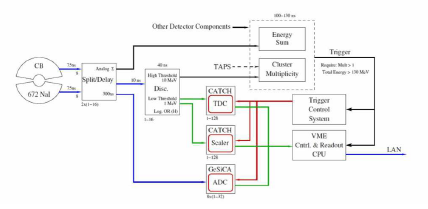
\includegraphics[scale=1.0]{pictures/png/cbelectronics.png}
\caption{Crystal Ball electronics \cite{krambrich}.}
\label{cbelectronics}
\end{center}
\end{figure}

\indent The integral of the pulse from each PMT was obtained from the F-ADCs, which sampled the shape of the signal with a frequency of 40 MHz. Since the DAQ was not prepared to handle such large volumes of data, only the integrals of pulses over three regions were taken. The integration is done over a time window of 750ns (30 signals). The first window was set to sample the pedestal whose signal is a convolution of remnant light and residual charge in the PMTs. The second window was set over the signal, and the third was set to evaluate the tail of the pulse. This set up allowed for the simultaneous measurement of the signal and the pedestal for every event, and with the dynamic subtraction of the pedestal from the signal, the energy resolution of the crystals could have been significantly improved.

\indent Contrary to the typical TDCs, which are started by a hit in a relevant detector and stopped by a logic pulse from the trigger, CATCH TDCs, developed for the Compass experiment at CERN, allow for multiple hits in TDCs \cite{gbruan}. Using a ~10GHz oscillator each TDC is running independently while the CERN-standard trigger control system synchronizes the signals in those TDCs. One of the TDCs is designated as a reference element and attached to the trigger. When an event passes the trigger threshold a logic pulse is sent to this reference TDC and the oscillator value is stored. When other TDCs record a hit, corresponding oscillator value is stored in a buffer. In order to extract the information on the timing of an event the oscillator value stored in the reference TDC has to be subtracted from the oscillator values recorded by other TDCs, the conversion rate of 117 ps/channel is then used \cite{lschmitt}.

\subsection{TAPS Electronics}

\indent The signals from the TAPS PMTs received similar treatment to those from Crystal Ball and were also split into three separate signals. One signal was directed to a TDC via a constant fraction discriminator (CFD), which analyzed the shape of the pulse and provided accurate timing information for the QDCs. The other two signals were fed to separate QDCs, one with integration time of 40ps, other with 200ps, this double integration allows for a pulse shape analysis.

\subsection{Triggering Electronics}

\indent While the event is being registered by DAQ, no other even is being recorded; this is defined as dead time. In order to reduce the effects of the dead time, a series of triggers were set up to limit the events read by DAQ only to those relevant to the experiment. Two LeCroy LRS 4805 logic units were used to define the conditions an event must satisfy in order to be recorded.

\indent The first level trigger for this experiment required the sum of energy deposited in all 672 NaI crystals to be greater than 40MeV. For the second level trigger, DAQ grouped NAI crystal into clusters of 16, and it was required that there were two hit clusters detected in the CB. When those two conditions were satisfied DAQ read the event and reset the electronics.


\section{Analysis code}

\indent Online analysis and monitoring of the data have been done using the AcquRoot framework. AcquRoot has been written in C++ specifically for the data analysis at MAMI, it uses libraries and tools of R00T \cite{john, root}. AcquRoot consists of three components, AcquDAQ Data Acquisition, AcquRoot Analysis and AcquMC Event Generator.

\indent Offline analysis was done using the a2GoAT framework(A2 Generation of Analysis Trees). In this framework AcquRoot is used to produce analysis trees containing only basic track information. The GoAT software package is then used to process those trees; here particle reconstruction, all the data checks and sorting is performed.

\chapter{Calibrations}

\indent This chapter addresses the calibrations of all the detectors. The process involved converting raw signals from the detectors into real physical quantities allowing for the energy, position and timing corrections to be determined and applied in the subsequent analysis.

\section{Tagger Energy Calibrations}

\indent The tagger energy calibration determines the relation between tagger channel number and electron energy. The calibrations were carried out by the colleagues at the University of Glasgow \cite{mcgeorge}.

\indent In order to make a tagger energy calibration, an incident MAMI electron beam of an energy of interest is bent in the magnetic field; for a 855MeV beam, field of ~1.025T is used. Then the magnetic field was varied in small steps to guide the beam through the focal plane and an energy measurement was taken at each step. Six different electron beam energies were used for the calibration, they ranged from 195.22MeV to 705.26 MeV, with the uncertainty of 0.16MeV; the uncertainty in the magnetic field was 0.01mT \cite{duncan}.

\indent The varying magnetic field required to sweep the beam across a given channel allowed for the determination of a position of a  hit in a FP detector with an accuracy of 0.05 channel width. Finally, in order to relate the the FP channel number to the electron energy a linear interpolation between different energies was used.

\section{Crystal Ball Calibrations}

\subsection{Clustering Algorithm}

\indent Photons entering Crystal Ball deposit their energy in the NaI crystals via electromagnetic showers which hit multiple crystals in each event.These groups of hit crystals are called clusters. The accurate analysis of the CB events required an algorithm which identifies the clusters and recovers information about the incident photon's energy and position from the energy deposited in the crystals within a cluster.

\indent First step in the analysis is to identify a crystal with the highest energy deposit, central crystal of the cluster, and it's 12 closest neighbours (Fig. \ref{cbcluster}). A hit in this central crystal provides the timing information for the event. The energies of the neighbouring crystals are scanned and if their energies are greater than the threshold energy of around 2MeV they are added to the cluster. Only 12 closest neighbours of the central crystal are considered in the algorithm because it has been confirmed that in 98\% of the cases the energy deposit of the shower triggers only 13 crystals \cite{claire}. Then the total energy of the cluster is obtained as:

\begin{equation}
E_{sum}=\Sigma_{k}E_{i}
\end{equation}

where, $E_{i}$ is the energy of the ith crystal in the cluster of k detector elements. Then the condition of the the total energy of the cluster being greater than 20MeV  is applied to suppress the effects of the background.

\indent The position of the hit is calculated as the weighted mean position given by the below equation:

\begin{equation}
r_{mean}=\frac{\Sigma_{k}\sqrt{E_{i}r_{i}}}{\Sigma_{k}\sqrt{E_{i}}}
\end{equation}

where, $E_{i}$ is the energy deposited in the ith crystal and $r_{i}$ is the position of the ith crystal in the cluster.

\begin{figure}[H]
\begin{center}
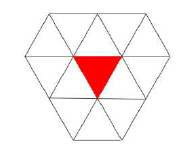
\includegraphics[scale=0.55]{cbcluster.png}
\caption{Schematic representation of a NaI cluster. The central triangle, shaded in red, depicts a triangular face of the NaI crystal and is the logical centre of the cluster. The other 12 triangles are its closest neighbours.}
\label{cbcluster}
\end{center}
\end{figure}

\subsection{Energy Calibration}

\indent Crystal Ball energy calibrations have been carried out by the colleagues from UCLA and Johanes Gutenberg Universitaet in Mainz \cite{marc}. The energy calibration of the Crystal Ball was performed in three steps; a low energy calibration - mainly important for the acquisition system was obtained, then a high energy calibration has been performed, and in the end, an energy scale factor has been applied to account for crystal thresholds and clustering algorythms.

\subsubsection{Low energy calibration}

\indent In this first step of the CB energy calibration, an $^{241}$Am/$^{9}$Be source was placed in the centre of the Crystal Ball \cite{marc}. The $\alpha$ decay of americium, and a subsequent capture of these particles by beryllium, triggers a series of reactions resulting in the excited state of $^{12}$C which decays to a ground state and emits a 4.438MeV photon in the process. This photon energy deposit in the NaI crystals has been used to adjust the gains of all PMTs, so that the detected peak was in the same position in the ADC spectra for all the detector elements.

\subsubsection{High energy calibration}

\indent The photons produced in meson decay have energies much higher than photons used in the low energy calibration, therefore the calibration for higher energy photons is also required. The $\pi^{0}->\gamma\gamma$ reaction have been used as a source of such photons. The invariant mass, M$_{\gamma\gamma}$, of two photons detected in the CB was reconstructed from the information on the photons measured energy and momentum and only the events with M$_{\gamma\gamma}$ within the mass of $\pi^{0}$ were selected, and the following selection cuts have been applied:

\begin{itemize}
\item no less than 70\% of the detected photon energy had to be deposited in a single NaI crystal. This criterium was decided upon to ensure the deposit in a single crystal dominated the cluster.
\item in order to ensure that the photons used for the calibration were of similar energy, the condition of having the energy difference between two photon clusters being less than 35\% of the total energy have been set up.
\item the tagged photon energy had to be less than 180MeV. This restriction constrained the energy range of the decay photons between 40MeV and 125MeV. Such energy cut favoured large opening angles between the photons, resulting in an even angular distributions in the lab.
\end{itemize}

\indent The invariant mass of $\pi^{0}$ has been reconstructed from the two photon decay, and a Gaussian function has been fitted. The mean of the fit, corresponding to M$_{\gamma\gamma}$ , has been compared to the mass of $\pi^{0}$. With this information a new gain factor, $G_{new}$, was obtained according to the below equation:

\begin{equation}
G_{new}=\frac{M_{\gamma\gamma}}{M_{\pi^{0}}}G_{old} [\frac{MeV}{channel}]
\end{equation}

where, $G_{old}$ is the gain factor used previously. Because the detected energy of the photon cluster depended both, on the central crystal and all the other crystals in the cluster a single set of calculation to obtain the new gain was not enough. Several iterations were required for M$_{\gamma\gamma}$ to correspond to M$_{\pi^{0}}$.

\subsubsection{Energy scaling factor}

\indent Because of the energy losses due to individual energy thresholds and the showers, the energy of the incident photons is not the same as the total energy of the cluster. To account for this in the analysis, another energy correction had to be applied. In order to ensure that the mass reconstructed from the decay of two photons was indeed the mass of $\pi^{0}$ meson, a scaling factor of 1.05 was applied to the data.

\subsubsection{Time walk correction}

\indent Because of the slow time response of the NaI crystals, 250ns \cite{knoll}, there arises a time difference between the small and large signals registering at the discriminator threshold. Therefore, the times reported by the TDCs required a correction to account for this time difference and therefore improve the CB time resolution (Fig. \ref{cbtimewalk}). The corrected time, $T_{corr}$, is defined as:

\begin{equation}
T_{corr}=T - r\sqrt{\frac{a_{0}}{a}}
\end{equation}

where, T is the measured time, $a_{0}$ is the discriminator's voltage, r is the rise time and a is the signal's amplitude.

\begin{figure}[H]
\begin{center}
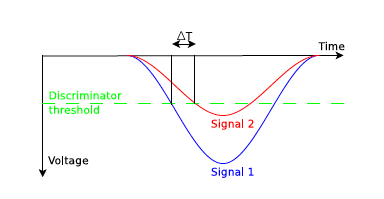
\includegraphics[scale=0.55]{cbtimewalk.png}
\caption{CB time walk.}
\label{cbtimewalk}
\end{center}
\end{figure}

\section{PID Calibration}

\subsection{PID azimuthal correction}

\indent In order to accurately determine the correlation between hits in the PID and Crystal Ball, the PID azimuthal angle ($\phi$) with respect to the Crystal Ball had to be measured. The steps taken to calculate the value of phi are as follows.
\indent First, only the events that triggered signal in one crystal in a CB cluster were selected. The reason for that was to limit the number of photons producing events in more than one crystal and therefore, ensure that only events with clearly determined angles were considered for the calibration. Another cut was made on those events to select only those with just a single reaction in the PID. This way the background due to multi-body final state interactions was highly reduced.
\indent The angular distribution of those events has been plotted for each PID element, which gave a single peak over the azimuthal range of each one (Fig. \ref{pidphi}). A 1D projection has been plotted for each PID element and a Gaussian function was fitted to the peak. Having 24 PID elements means that each of them occupies 15$\deg$ of the total azimuthal coverage. Therefore, a linear fit with a fixed gradient could have been used to accurately determine the PID azimuthal correction (Fig. \ref{pidphi2}).

\begin{figure}[H]
\begin{center}
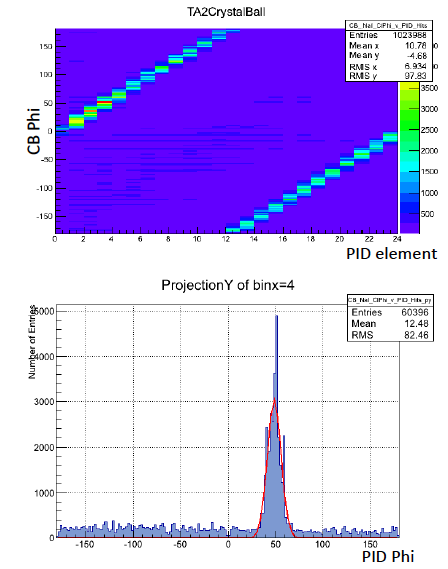
\includegraphics[scale=0.55]{pidphi.png}
\caption{Plot of Phi position in CB cluster vs hit in PID (top) and Gaussian fit to the projection of PID element 4 over the azimuthal range (bottom).}
\label{pidphi}
\end{center}
\end{figure}

\begin{figure}[H]
\begin{center}
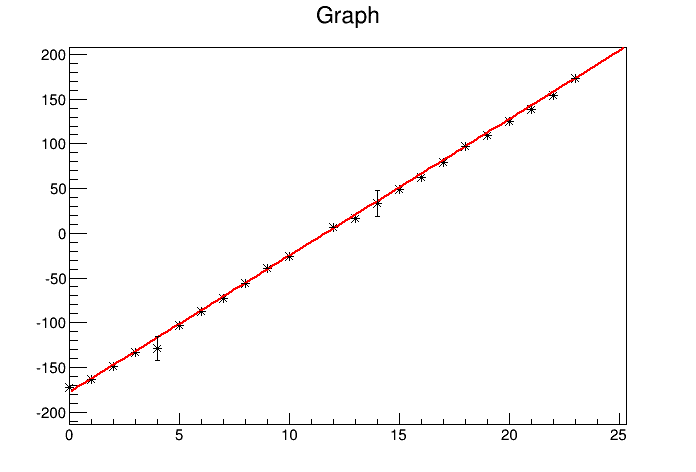
\includegraphics[scale=0.4]{pidcali4.png}
\caption{PID azimuthal correction - linear fit.}
\label{pidphi2}
\end{center}
\end{figure}

\subsection{PID energy correction}

\indent The energy calibration employed banana ($\Delta$E-E) plots described earlier and raw signal from PID ADCs. The banana plots were divided into 10MeV energy bins and projected onto the y-axis (Fig. \ref{bananacali}). Those projections featured two peaks, first one corresponding to the pion and second one representing proton ridges. The latter was fitted with a Gaussian function and the value of the mean has been extracted (Fig. \ref{bananagaus}). This step has been performed for all the energy bins in the range of 20-300MeV. Similarly, the G4 simulated data had the same procedure applied. Subsequently, the means of the Gaussian functions for the experimental data have been plotted against corresponding means for the simulated data and a linear fit has been used to determine the gain for the calibration (Fig. \ref{bananagaus}).

\begin{figure}[H]
\begin{center}
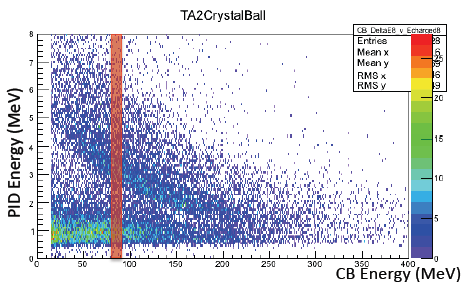
\includegraphics[scale=0.6]{bananacali.png}
\caption{$\Delta$E-E plots of PID vs CB energy deposits. Example10MeV energy bin shaded in red.}
\label{bananacali}
\end{center}
\end{figure}

\begin{figure}[H]
\begin{center}
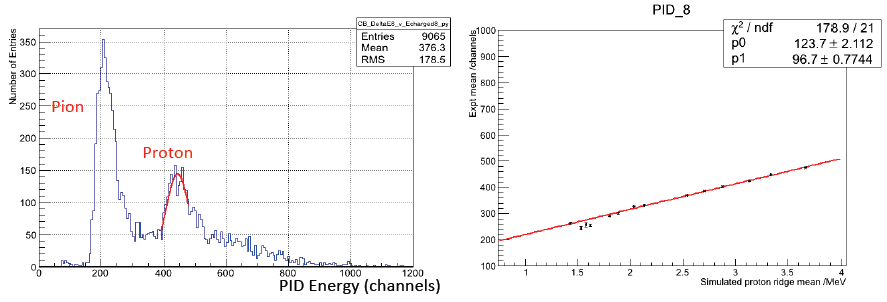
\includegraphics[scale=0.5]{bananagaus.png}
\caption{Gaussian function fitted to the proton peak (left) and linear fit to the Gaussian means (right).}
\label{bananagaus}
\end{center}
\end{figure}

\indent The offset for the calibration has been obtained from the analysis of the raw ADC signal for each PID element. The first peak in the ADC spectrum (Figure 6) represents the pedestal position. A Gaussian function has been fitted to this peak and the value of the mean has been determined. This value is equivalent to the offset for the calibration.

\subsection{PID time calibration}

\indent Accurate information about timing of the events, obtained with the TDCs, is essential part of the data analysis. Timing coincidence allows for correlation of coincidence particles between different detectors; it is used in clustering algorithm of the Crystal Ball, and enables particle identification in TAPS, therefore allowing for the association of a hit in FPD with an even in CB/TAPS detectors. The principles followed for time calibration of the various detectors are the same, therefore, only PID time calibration will be described in more detail below.

\indent The TDC spectrum of each PID element was fitted with a Gaussian and a value of the means for all the elements have been extracted (Fig. \ref{pidtdcgaus}). These values have been used to determine the offset in the calibration and align the peaks of all the detector elements in the timing spectrum (Fig. \ref{pidtdcoffset}). The misalignment for the PID element 17 is caused by the malfunctioning PID element (Fig. \ref{pidtdcgaus16}).

\begin{figure}[H]
\begin{center}
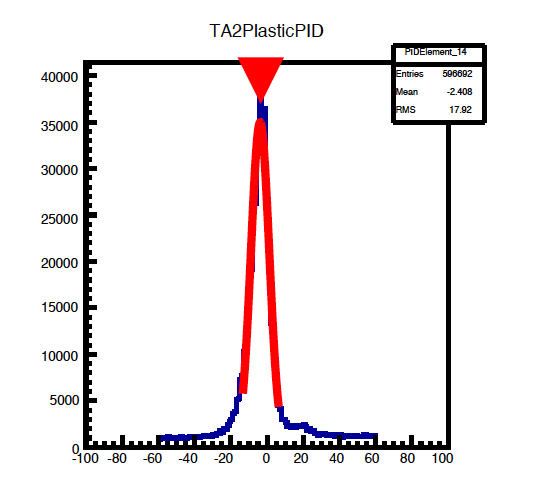
\includegraphics[scale=0.4]{pidtdcgaus.png}
\caption{Gaussian fit to PID-element 14.}
\label{pidtdcgaus}
\end{center}
\end{figure}

\begin{figure}[H]
\begin{center}
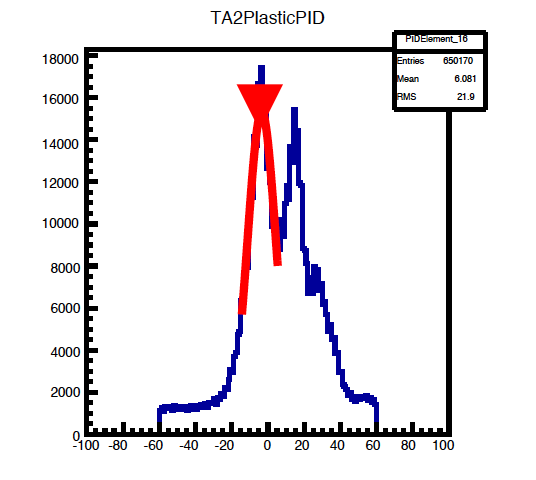
\includegraphics[scale=0.4]{pidtdcgaus16.png}
\caption{Gaussian fit to PID-element 16. The TDC spectrum of the malfunctioning PID element.}
\label{pidtdcgaus16}
\end{center}
\end{figure}

%\begin{figure}[H]
%\begin{centre}
%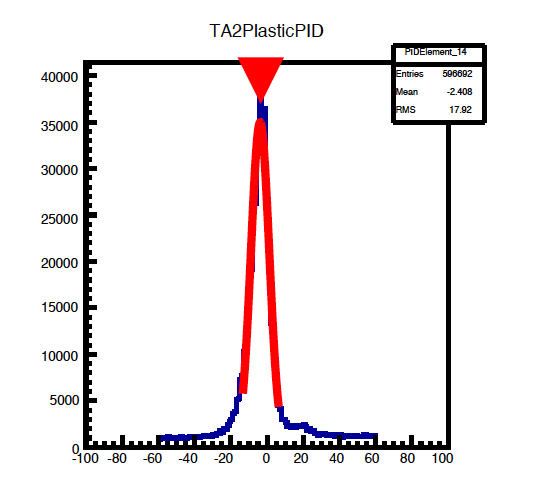
\includegraphics[scale=0.55]{pidtdcgaus.png}
%\caption{Gaussian fit to PID-element 14.}
%\label{pidtdcoffset}
%\end{center}
%\end{figure}

%\begin{figure}[H]
%\begin{centre}
%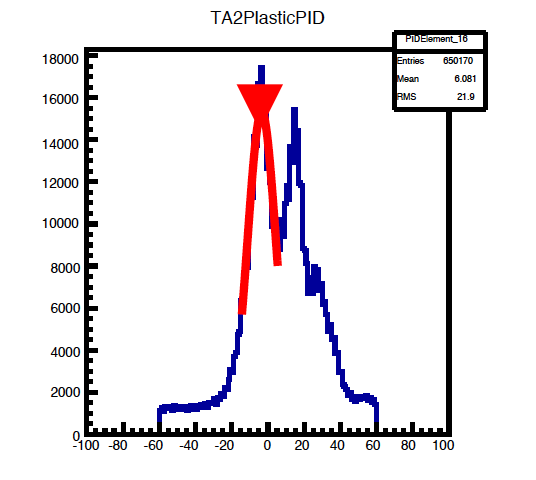
\includegraphics[scale=0.55]{pidtdcgaus16.png}
%\caption{Gaussian fit to PID-element 16. The TDC spectrum of the malfunctioning PID element.}
%\label{pidtdcoffset16}
%\end{center}
%\end{figure}

\begin{figure}[H]
\begin{center}
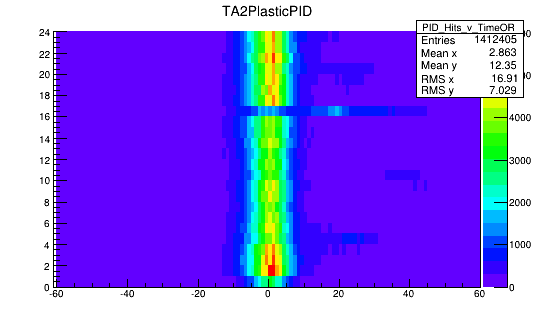
\includegraphics[scale=0.55]{pidtdcoffset.png}
\caption{Time alignment of all PID elements.}
\label{pidtdcoffset}
\end{center}
\end{figure}

\section{TAPS Calibration}

\indent The calibration of the TAPS BaF$_{2}$ crystals employed cosmic rays using the mean deposited energy of the minimum ionising muons equal to 37.7MeV \cite{roebig}. For each of the BaF$_{2}$ crystals' PMTs the position of the energy peak has been adjusted so it was at the same ADC position for all detector elements, and the channel number corresponding to the mean peak position was determined.

\indent Using a similar technique to that employed in the CB calibrations, the correction for the gain was obtained. However, because detection of two photons from the $\pi^{0}$ in TAPS is very rare, the events having one photon detected in TAPS and one in CB were chosen. Detailed procedure of this calibration can be found in \cite{lemmer}.

\indent The procedure to calibrate plastic Veto was similar to the one used to calibrate PID. The pedestal positions were obtained from the raw ADC spectra and the gain was determined by comparing the experimental mean position of the proton peak in the Veto to the simulated data. Details of this method can be found in reference \cite{gessler}

\section{Target Position Correction}


   
%\section{section name}

%some shit

%\section{section name}

%\chapter{Calibrations}

\indent This chapter addresses the calibrations of all the detectors. The process involved converting raw signals from the detectors into real physical quantities allowing for the energy, position and timing corrections to be determined and applied in the subsequent analysis.

\section{Tagger Energy Calibrations}

\indent The tagger energy calibration determines the relation between tagger channel number and electron energy. The calibrations were carried out by the colleagues at the University of Glasgow \cite{mcgeorge}.

\indent In order to make a tagger energy calibration, an incident MAMI electron beam of an energy of interest is bent in the magnetic field; for a 855MeV beam, field of ~1.025T is used. Then the magnetic field was varied in small steps to guide the beam through the focal plane and an energy measurement was taken at each step. Six different electron beam energies were used for the calibration, they ranged from 195.22MeV to 705.26 MeV, with the uncertainty of 0.16MeV; the uncertainty in the magnetic field was 0.01mT \cite{duncan}.

\indent The varying magnetic field required to sweep the beam across a given channel allowed for the determination of a position of a  hit in a FP detector with an accuracy of 0.05 channel width. Finally, in order to relate the the FP channel number to the electron energy a linear interpolation between different energies was used.

\section{Crystal Ball Calibrations}

\subsection{Clustering Algorithm}

\indent Photons entering Crystal Ball deposit their energy in the NaI crystals via electromagnetic showers which hit multiple crystals in each event.These groups of hit crystals are called clusters. The accurate analysis of the CB events required an algorithm which identifies the clusters and recovers information about the incident photon's energy and position from the energy deposited in the crystals within a cluster.

\indent First step in the analysis is to identify a crystal with the highest energy deposit, central crystal of the cluster, and it's 12 closest neighbours (Fig. \ref{cbcluster}). A hit in this central crystal provides the timing information for the event. The energies of the neighbouring crystals are scanned and if their energies are greater than the threshold energy of around 2MeV they are added to the cluster. Only 12 closest neighbours of the central crystal are considered in the algorithm because it has been confirmed that in 98\% of the cases the energy deposit of the shower triggers only 13 crystals \cite{claire}. Then the total energy of the cluster is obtained as:

\begin{equation}
E_{sum}=\Sigma_{k}E_{i}
\end{equation}

where, $E_{i}$ is the energy of the ith crystal in the cluster of k detector elements. Then the condition of the the total energy of the cluster being greater than 20MeV  is applied to suppress the effects of the background.

\indent The position of the hit is calculated as the weighted mean position given by the below equation:

\begin{equation}
r_{mean}=\frac{\Sigma_{k}\sqrt{E_{i}r_{i}}}{\Sigma_{k}\sqrt{E_{i}}}
\end{equation}

where, $E_{i}$ is the energy deposited in the ith crystal and $r_{i}$ is the position of the ith crystal in the cluster.

\begin{figure}[H]
\begin{center}
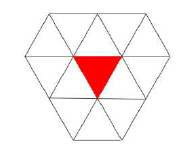
\includegraphics[scale=0.55]{cbcluster.png}
\caption{Schematic representation of a NaI cluster. The central triangle, shaded in red, depicts a triangular face of the NaI crystal and is the logical centre of the cluster. The other 12 triangles are its closest neighbours.}
\label{cbcluster}
\end{center}
\end{figure}

\subsection{Energy Calibration}

\indent Crystal Ball energy calibrations have been carried out by the colleagues from UCLA and Johanes Gutenberg Universitaet in Mainz \cite{marc}. The energy calibration of the Crystal Ball was performed in three steps; a low energy calibration - mainly important for the acquisition system was obtained, then a high energy calibration has been performed, and in the end, an energy scale factor has been applied to account for crystal thresholds and clustering algorythms.

\subsubsection{Low energy calibration}

\indent In this first step of the CB energy calibration, an $^{241}$Am/$^{9}$Be source was placed in the centre of the Crystal Ball \cite{marc}. The $\alpha$ decay of americium, and a subsequent capture of these particles by beryllium, triggers a series of reactions resulting in the excited state of $^{12}$C which decays to a ground state and emits a 4.438MeV photon in the process. This photon energy deposit in the NaI crystals has been used to adjust the gains of all PMTs, so that the detected peak was in the same position in the ADC spectra for all the detector elements.

\subsubsection{High energy calibration}

\indent The photons produced in meson decay have energies much higher than photons used in the low energy calibration, therefore the calibration for higher energy photons is also required. The $\pi^{0}->\gamma\gamma$ reaction have been used as a source of such photons. The invariant mass, M$_{\gamma\gamma}$, of two photons detected in the CB was reconstructed from the information on the photons measured energy and momentum and only the events with M$_{\gamma\gamma}$ within the mass of $\pi^{0}$ were selected, and the following selection cuts have been applied:

\begin{itemize}
\item no less than 70\% of the detected photon energy had to be deposited in a single NaI crystal. This criterium was decided upon to ensure the deposit in a single crystal dominated the cluster.
\item in order to ensure that the photons used for the calibration were of similar energy, the condition of having the energy difference between two photon clusters being less than 35\% of the total energy have been set up.
\item the tagged photon energy had to be less than 180MeV. This restriction constrained the energy range of the decay photons between 40MeV and 125MeV. Such energy cut favoured large opening angles between the photons, resulting in an even angular distributions in the lab.
\end{itemize}

\indent The invariant mass of $\pi^{0}$ has been reconstructed from the two photon decay, and a Gaussian function has been fitted. The mean of the fit, corresponding to M$_{\gamma\gamma}$ , has been compared to the mass of $\pi^{0}$. With this information a new gain factor, $G_{new}$, was obtained according to the below equation:

\begin{equation}
G_{new}=\frac{M_{\gamma\gamma}}{M_{\pi^{0}}}G_{old} [\frac{MeV}{channel}]
\end{equation}

where, $G_{old}$ is the gain factor used previously. Because the detected energy of the photon cluster depended both, on the central crystal and all the other crystals in the cluster a single set of calculation to obtain the new gain was not enough. Several iterations were required for M$_{\gamma\gamma}$ to correspond to M$_{\pi^{0}}$.

\subsubsection{Energy scaling factor}

\indent Because of the energy losses due to individual energy thresholds and the showers, the energy of the incident photons is not the same as the total energy of the cluster. To account for this in the analysis, another energy correction had to be applied. In order to ensure that the mass reconstructed from the decay of two photons was indeed the mass of $\pi^{0}$ meson, a scaling factor of 1.05 was applied to the data.

\subsubsection{Time walk correction}

\indent Because of the slow time response of the NaI crystals, 250ns \cite{knoll}, there arises a time difference between the small and large signals registering at the discriminator threshold. Therefore, the times reported by the TDCs required a correction to account for this time difference and therefore improve the CB time resolution (Fig. \ref{cbtimewalk}). The corrected time, $T_{corr}$, is defined as:

\begin{equation}
T_{corr}=T - r\sqrt{\frac{a_{0}}{a}}
\end{equation}

where, T is the measured time, $a_{0}$ is the discriminator's voltage, r is the rise time and a is the signal's amplitude.

\begin{figure}[H]
\begin{center}
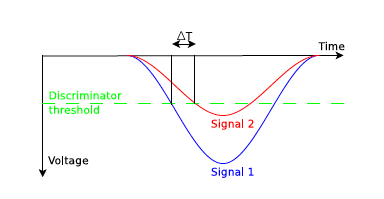
\includegraphics[scale=0.55]{cbtimewalk.png}
\caption{CB time walk.}
\label{cbtimewalk}
\end{center}
\end{figure}

\section{PID Calibration}

\subsection{PID azimuthal correction}

\indent In order to accurately determine the correlation between hits in the PID and Crystal Ball, the PID azimuthal angle ($\phi$) with respect to the Crystal Ball had to be measured. The steps taken to calculate the value of phi are as follows.
\indent First, only the events that triggered signal in one crystal in a CB cluster were selected. The reason for that was to limit the number of photons producing events in more than one crystal and therefore, ensure that only events with clearly determined angles were considered for the calibration. Another cut was made on those events to select only those with just a single reaction in the PID. This way the background due to multi-body final state interactions was highly reduced.
\indent The angular distribution of those events has been plotted for each PID element, which gave a single peak over the azimuthal range of each one (Fig. \ref{pidphi}). A 1D projection has been plotted for each PID element and a Gaussian function was fitted to the peak. Having 24 PID elements means that each of them occupies 15$\deg$ of the total azimuthal coverage. Therefore, a linear fit with a fixed gradient could have been used to accurately determine the PID azimuthal correction (Fig. \ref{pidphi2}).

\begin{figure}[H]
\begin{center}
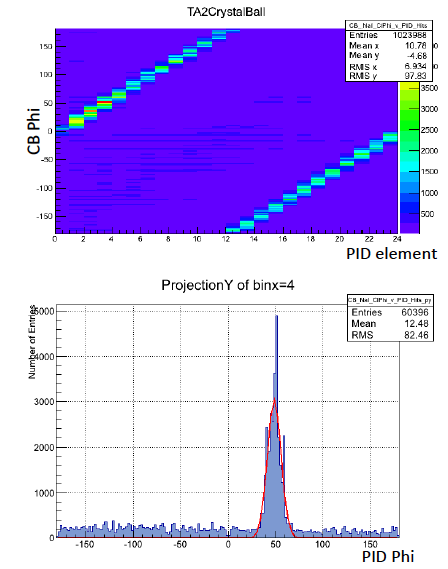
\includegraphics[scale=0.55]{pidphi.png}
\caption{Plot of Phi position in CB cluster vs hit in PID (top) and Gaussian fit to the projection of PID element 4 over the azimuthal range (bottom).}
\label{pidphi}
\end{center}
\end{figure}

\begin{figure}[H]
\begin{center}
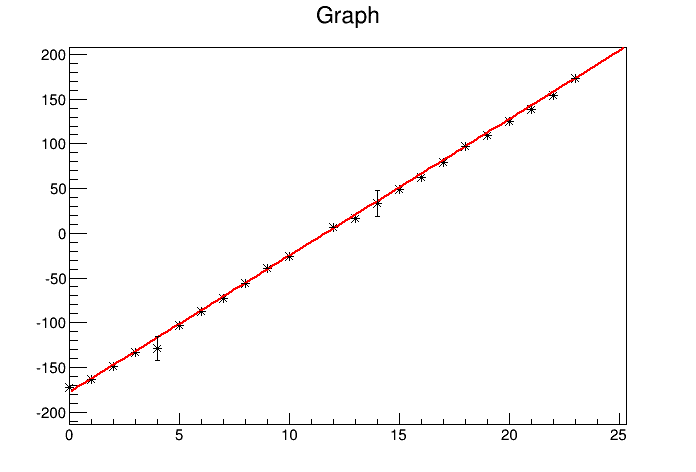
\includegraphics[scale=0.4]{pidcali4.png}
\caption{PID azimuthal correction - linear fit.}
\label{pidphi2}
\end{center}
\end{figure}

\subsection{PID energy correction}

\indent The energy calibration employed banana ($\Delta$E-E) plots described earlier and raw signal from PID ADCs. The banana plots were divided into 10MeV energy bins and projected onto the y-axis (Fig. \ref{bananacali}). Those projections featured two peaks, first one corresponding to the pion and second one representing proton ridges. The latter was fitted with a Gaussian function and the value of the mean has been extracted (Fig. \ref{bananagaus}). This step has been performed for all the energy bins in the range of 20-300MeV. Similarly, the G4 simulated data had the same procedure applied. Subsequently, the means of the Gaussian functions for the experimental data have been plotted against corresponding means for the simulated data and a linear fit has been used to determine the gain for the calibration (Fig. \ref{bananagaus}).

\begin{figure}[H]
\begin{center}
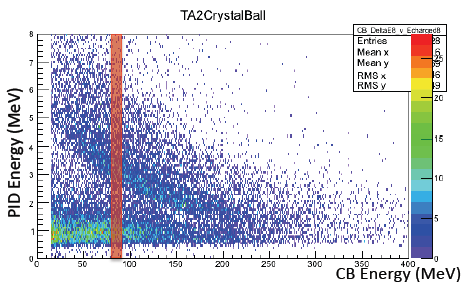
\includegraphics[scale=0.6]{bananacali.png}
\caption{$\Delta$E-E plots of PID vs CB energy deposits. Example10MeV energy bin shaded in red.}
\label{bananacali}
\end{center}
\end{figure}

\begin{figure}[H]
\begin{center}
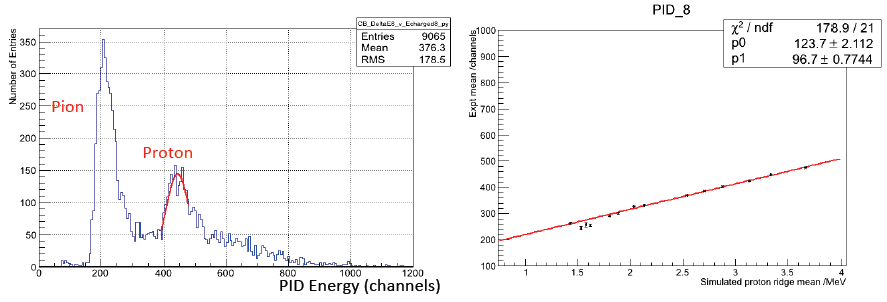
\includegraphics[scale=0.5]{bananagaus.png}
\caption{Gaussian function fitted to the proton peak (left) and linear fit to the Gaussian means (right).}
\label{bananagaus}
\end{center}
\end{figure}

\indent The offset for the calibration has been obtained from the analysis of the raw ADC signal for each PID element. The first peak in the ADC spectrum (Figure 6) represents the pedestal position. A Gaussian function has been fitted to this peak and the value of the mean has been determined. This value is equivalent to the offset for the calibration.

\subsection{PID time calibration}

\indent Accurate information about timing of the events, obtained with the TDCs, is essential part of the data analysis. Timing coincidence allows for correlation of coincidence particles between different detectors; it is used in clustering algorithm of the Crystal Ball, and enables particle identification in TAPS, therefore allowing for the association of a hit in FPD with an even in CB/TAPS detectors. The principles followed for time calibration of the various detectors are the same, therefore, only PID time calibration will be described in more detail below.

\indent The TDC spectrum of each PID element was fitted with a Gaussian and a value of the means for all the elements have been extracted (Fig. \ref{pidtdcgaus}). These values have been used to determine the offset in the calibration and align the peaks of all the detector elements in the timing spectrum (Fig. \ref{pidtdcoffset}). The misalignment for the PID element 17 is caused by the malfunctioning PID element (Fig. \ref{pidtdcgaus16}).

\begin{figure}[H]
\begin{center}
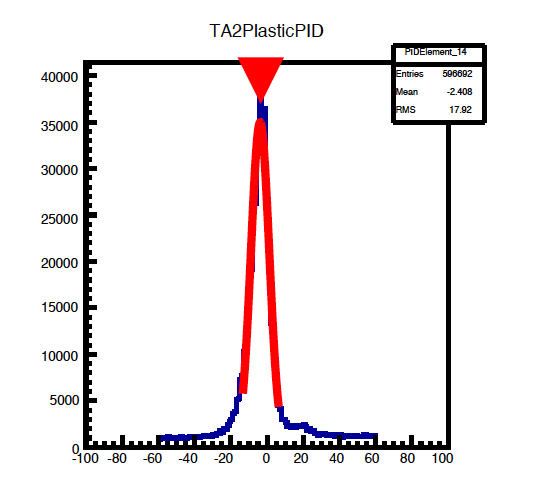
\includegraphics[scale=0.4]{pidtdcgaus.png}
\caption{Gaussian fit to PID-element 14.}
\label{pidtdcgaus}
\end{center}
\end{figure}

\begin{figure}[H]
\begin{center}
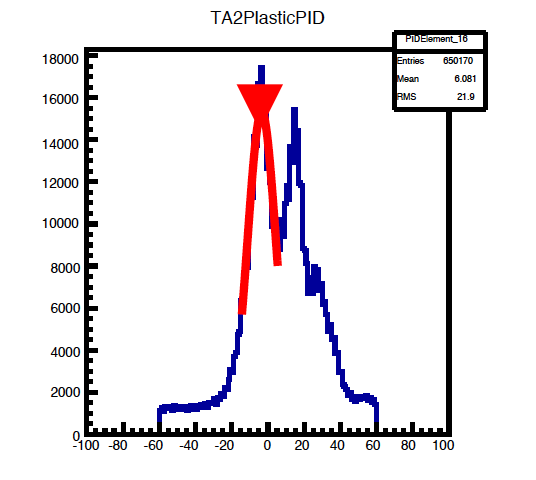
\includegraphics[scale=0.4]{pidtdcgaus16.png}
\caption{Gaussian fit to PID-element 16. The TDC spectrum of the malfunctioning PID element.}
\label{pidtdcgaus16}
\end{center}
\end{figure}

%\begin{figure}[H]
%\begin{centre}
%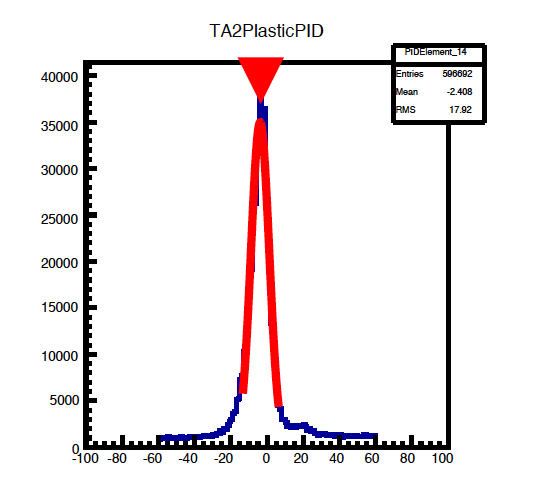
\includegraphics[scale=0.55]{pidtdcgaus.png}
%\caption{Gaussian fit to PID-element 14.}
%\label{pidtdcoffset}
%\end{center}
%\end{figure}

%\begin{figure}[H]
%\begin{centre}
%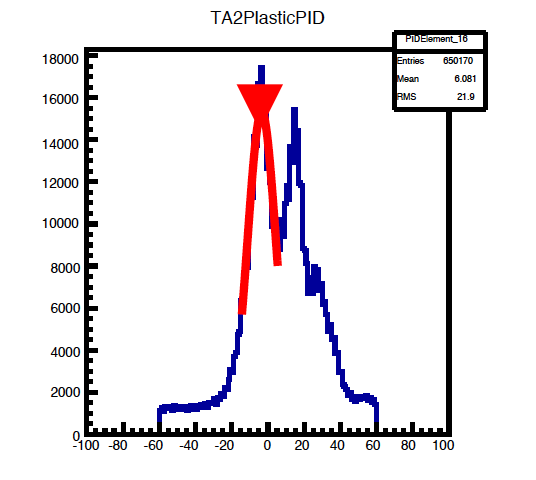
\includegraphics[scale=0.55]{pidtdcgaus16.png}
%\caption{Gaussian fit to PID-element 16. The TDC spectrum of the malfunctioning PID element.}
%\label{pidtdcoffset16}
%\end{center}
%\end{figure}

\begin{figure}[H]
\begin{center}
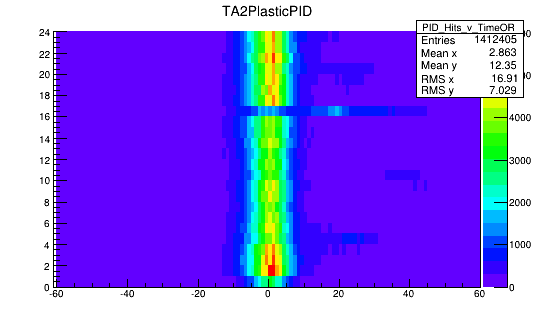
\includegraphics[scale=0.55]{pidtdcoffset.png}
\caption{Time alignment of all PID elements.}
\label{pidtdcoffset}
\end{center}
\end{figure}

\section{TAPS Calibration}

\indent The calibration of the TAPS BaF$_{2}$ crystals employed cosmic rays using the mean deposited energy of the minimum ionising muons equal to 37.7MeV \cite{roebig}. For each of the BaF$_{2}$ crystals' PMTs the position of the energy peak has been adjusted so it was at the same ADC position for all detector elements, and the channel number corresponding to the mean peak position was determined.

\indent Using a similar technique to that employed in the CB calibrations, the correction for the gain was obtained. However, because detection of two photons from the $\pi^{0}$ in TAPS is very rare, the events having one photon detected in TAPS and one in CB were chosen. Detailed procedure of this calibration can be found in \cite{lemmer}.

\indent The procedure to calibrate plastic Veto was similar to the one used to calibrate PID. The pedestal positions were obtained from the raw ADC spectra and the gain was determined by comparing the experimental mean position of the proton peak in the Veto to the simulated data. Details of this method can be found in reference \cite{gessler}

\section{Target Position Correction}


   
%\section{section name}

%some shit

%\section{section name}
 etc....... named as the bit before the ".tex" in the folder


\small{
\singlespacing

%\bibliographystyle{these} %optional
%\bibliography{refs}


}

\end{document}




